\lohead{Hörmann Stefan}
\chapter{Mechanik}

\section{Einleitung}

\section{Anforderung}
\label{sec:Anforderung}
Die Arbeit des mechanischen Teiles besteht darin, eine Maschine,
die Spielkarten mischen und ausgeben kann zu entwerfen, zu konstruieren
und einen Teilaufbau durchzuführen. Die Maschine sollte in der Lage
sein 20 Spielkarten zu mischen und diese nach einem Spielmodus der
zuvor am LCD gewählt wurde auszugeben. Das Ziel ist es, die Spielkarten
optimal zu mischen, aber die Maschine dennoch kompakt und optisch
ansprechen zu entwerfen. Im weiteren sollte der Mischvorgang und die
Ausgabe der Karten nicht zu lange dauern. Die Teile der Maschine
sollten so konstruiert werden, dass sie kostengünstig produziert
werden können. Zum Schluss sollte noch ein Teilaufbau der Maschine
geschehen, um die Funktionalität der einzelnen Bereiche zu testen
und gegebenfalls zu verbessern.

\section{Problemstellungen}
Ein Problem ist das begrenzte Budget unseres Teams, somit sind
wir auf gewisse Produktionsarten unserer Bauteile beschränkt.
Dies hat zur Folge, dass die Bauteile oft sehr simpel sind um
sie leichter zu konstruieren. Die Oberfläche der Karten ist ein
weiteres Problem, da diese sich nicht immer separieren lassen, dies
verursacht, dass oft zwei oder mehrere Karten auf einmal genommen
werden und das Konzept des optimalen Mischens zerstört.

\section{Konzepte}

\subsection{Anforderungen}

\begin{enumerate}
    \item \textbf{Kosten}  \\
    Der Automat sollte möglichst kostengünstig produziert werden,
    da das vorhandene Budget gering ist. Dies hat zur Folge das keine teuren Motoren
    oder ähnliche Bauteile zum Einsatz kommen können und keine teuren Bauteile produziert
    werden können.
    \item \textbf{Schnelligkeit} \\
    Um ein gutes Spielerlebnis zu garantieren, sollte der Automat keine
    langen Mischzeit besitzen. Die Dauer in der man die Karten einführt und auf den
    Mischen-Button klickt bis hin zur Ausgabe der ersten Karte sollte möglichst gering sein.
    \item \textbf{Mischgenauigkeit} \\
    Die Mischgenauigkeit ist die am schwersten gewichtete Anforderung,
    da es das Ziel ist ein optimales Mischen der Spielkarten zu erreichen, sollte
    diese Anforderung mit größter Wichtigkeit erfüllt werden.
    \item \textbf{Optik und Größe} \\
    Die Optik des Automaten soll schlicht gehalten werden, jedoch sollte
    sie dennoch auf Messen und andere Ausstellungen präsentierbar sein. Der Automat
    sollte jedoch auch stabil konstruiert werden, muss aber dennoch mobil bleiben und
    darf eine gewisse Größe nicht Überschreiten.
\end{enumerate}

\subsection{Variantenvergleich}
Um alle oben angegebenen Anforderungen zu erfüllen, wurden mehrere Konzepte entworfen und diese verglichen.

\subsubsection{Variante 1 - Linearachsen}


\begin{figure}[hb]
    \centering
    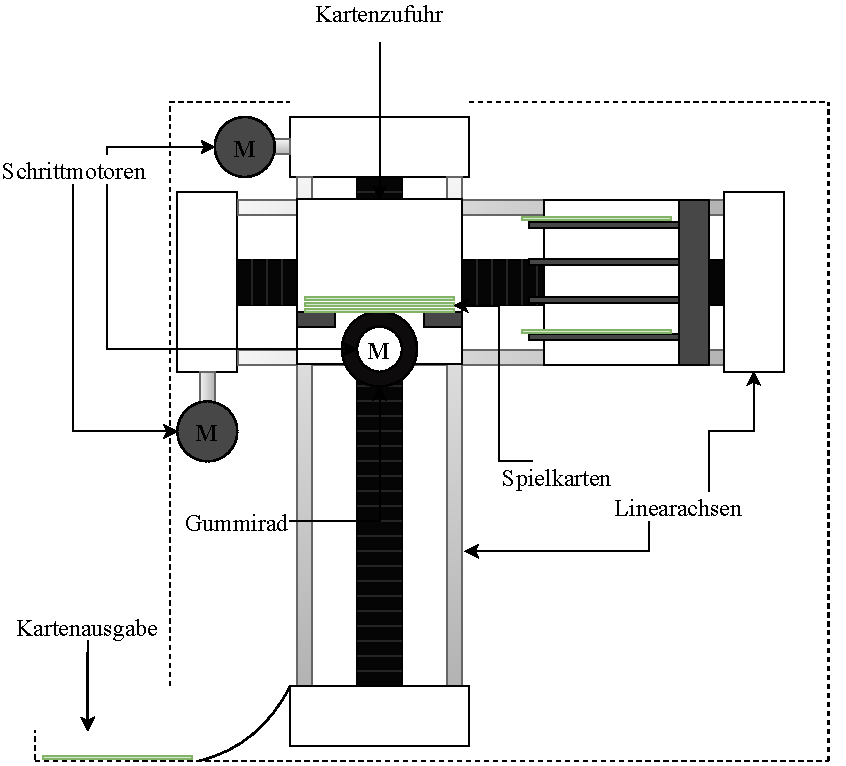
\includegraphics[scale=0.5,page=1]{fig/mech/Version1}
    \caption{Variante 1}
\end{figure}


Das erste Konzept würde mit zwei Linearachsen realisiert werden, diese wären im rechten Winkel zueinander
angeordnet. Die Senkrechte Linearachse ist mit einer Halterung versehen, diese Halterung ist in der Lage
ein Kartendeck aufzunehmen und die unterste Karte mithilfe eines Ausgaberades weiterzubefördern. Die zweite
Linearachse besitzt 4 Fächer in der die Karten von der ersten Linearachsenausgabe zufällig befördert werden.
Dies wird realisiert indem die erste Linearachse bei jeder Ausgabe zufällig das Fach durch hinauf und
hinabfahren wechselt. Befinden sich alle Karten im Lager, so fährt die erste Linearachse nach unten, danach
fährt die zweite Linearachse impulsiv nach links, um die Karten aus dem Lager zu befördern. Diese fallen
Senkrecht in das Lager der ersten Linearachse, wo sie nun zum Ausgeben durch das Ausgaberad bereit liegen. \\



Durch die schnelle Bewegung der Linearachsen ist es möglich einen schnellen Mischprozess zu erreichen,
auch die Tatsache das es nur ein rotierendes Rad gibt und zwei Bewegliche Linearachsen führt dazu, das
Fehler bei Bewegungen nur selten Auftreten. Jedoch besteht durch den hohen Aufbau der Maschine und durch die hohe
Position der zweiten Linearachse die sich horizontal bewegt die Gefahr des umkippens der Maschine, und somit ist
keine stabilität mehr gegeben. Der Preis der Linearachsen ist ein weiterer Nachteil dieses Konzeptes, eine Linearachse
die unsere Anforderungen entspricht, wäre mit Motor und Schlitten zu teuer für unser Budget. \\

\textbf{Vorteile:}
\begin{itemize}
    \item schnelles Mischen
    \item wenige Fehlerquellen
\end{itemize}
\textbf{Nachteile:}
\begin{itemize}
    \item teuer
    \item großer Aufbau %Genaueres Beschreiben der Vor und Nachteile?
    \item instabil
\end{itemize}

\subsubsection{Variante 2 - Lagerrad mit Asugaberäder}

\begin{figure}[hb]
    \centering
    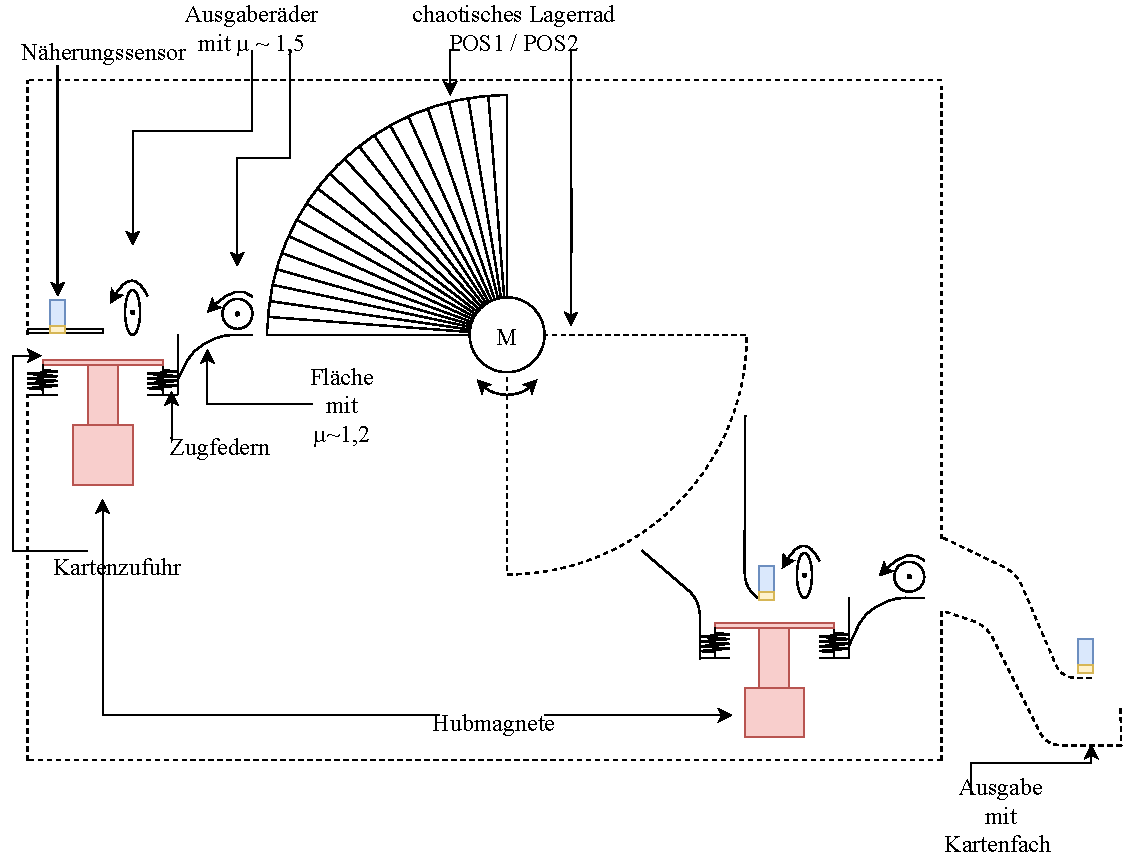
\includegraphics[scale=0.5,page=1]{fig/mech/Version2}
    \caption{Variante 2}
\end{figure}

Beim zweiten Konzept wird als Lager ein virtel eines Zylinders benutzt. In diesem befinden
sich verschidene Fächer in der die Karten eingelagert werden. Dieser wird mit einem Motor betrieben
und dreht sich somit in die vorgegebenen Positionen um das Einlagern und das Ausgeben der Karten zu ermöglichen.
Die Karteneingabe erfolgt über einen Schlitz in der Frontplatte der Maschine, dort befindet sich ein Hubmagnet der die Karten
zum weiterbefördern nach oben drückt. Ein Kapazitiver Sensor sorgt dafür, das scihergestellt werden kann, dass sich Karten auf dem Hubmagnet befinden.
Um eine Karte in das Lager zu befördern wird der Hubmagnet eingeschaltet und drückt das Kartendeck auf das erste Ausgaberad, um die Kraft des Hubmagnetes zu minimieren sind Zugfedern angebracht.
Das Ausgaberad befördert eine Karte weiter vor zum zweiten Ausgabrad welches weiderum sicherstellt das nur eine Karten in das Lagerrad transportiert wird.
Danach dreht das Lagerrad auf eine andere zufällig ausgewählte Position. Dieser Prozess wird solange wiederholt bis alle Karten des Kartendecks sich im Lagerrad befinden.
Befinden sich alle Karten im Lagerrad, so dreht sich dieses mit einer hochen Geschwindigkeit und wirft somit die Karten auf der Hinterseite der Maschine in eine Auffangführung. %Ist Geschwindigkeit der richtige Begriff? Eher Moment oder Drehzahl?
Diese Auffangsführung befördert die Karten in einen gleichen Mechanismus wie bei der Vorderseite der Maschine, in der sie von einem Hubmagenten nach oben gedrückt werden und von zwei Ausgaberädern zur
Kartenentnahme geschoben werden. Da die Karten zum Schluss nach einem Spielmodus und somit in einer bestimmten Anzahl Ausgegeben werden, befindet sich ein Kapazitiver Sensor auch bei der Ausgabe der Karten,
dieser soll überprüfen ob die Karten von dem Spiler berreits genommen wurden oder nicht.\\

Durch den niedrigen Aufbau der durch ein "Fließbandartiges" befördern der Karten erreicht wird, besitzt die Maschine ein hohes Maß an stabilität, jedoch ensteht dadurch auch der Nachteil
dass die Maschine sehr lang wird. Da dieses Konzept 5 bewegliche Räder besitzt sowie zwei Hubmagneten ist es anfällig für Fehler beim Bewegungsablauf. Auch kann nicht garantiert werden
dass nur eine Karte in das Lagerrad befördert wird, dies würd das Konzept des optimalen Mischens zerstören. Die vielen Bauteile führen auch zu teureren Anschaffungskosten, die wir stark vermeiden möchten.\\

\textbf{Vorteile:}
\begin{itemize}
    \item stabil
    \item niedriger Aufbau
\end{itemize}
\textbf{Nachteile:}
\begin{itemize}
    \item lange Gesamtgröße
    \item viele bewegliche Bauteile / Fehlerquellen
\end{itemize}

\subsubsection{Variante 3 - Lagerrad mit Saugnäpfe}

\begin{figure}[H]
    \centering
    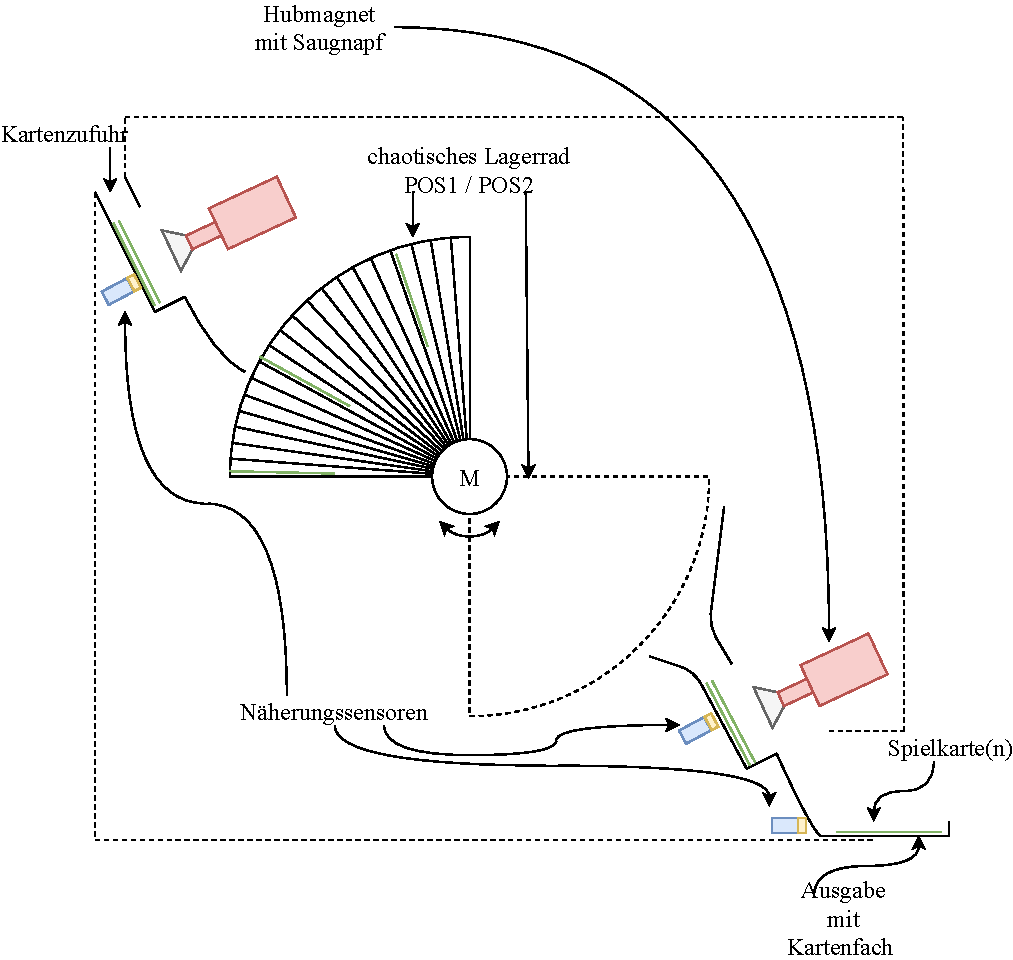
\includegraphics[scale=0.5,page=1]{fig/mech/Version3}
    \caption{Variante 3}
\end{figure}

Das dritte Konzept besitzt ein identes Lagersystem wie das zweite Konzept, ein Lagerrad das in Fächer unterteilt ist und über einen Moter diverse Positionen einnehmen kann.
Das Kartendeck wird in den oberen / vorderen Anfang der Maschine eingeführt. Dort liegt es schräg in einem Winkel von ca. 60°. Um sicherzustellen das sich Karten in dieser Halterung befinden
ist ein Kapazitiver Sensor an der Unterseite angebracht. Ein Hubmagnet der im rechten Winkel zu den Karten über der Halterng angebracht ist, saugt jede Karte einzeln an indem ein Saugnapf der an einem Hubmagneten
befestigt ist heruntergedrückt wird. Ist die Karte angesaugt, so wird der Hubmagnet von einer Feder in seine Ausgangsstellung zurückgebracht, dabei wird die Spielkarte durch eine Platte abgestreift und fliegt somit in das Lager des
Lagerrades hinein. Dieser Prozess wird solange wiederholt bis sich alle Spilkarten des Kartendecks im Lagerrad befinden. Sind alle Karten im Lagerrad so dreht sich dieses und wirft die Karten auf der Rückseite der Maschine in ein Führung
die die Karten in eine zweite Halterung befördern. Diese zweite Halterung ist ident Aufgebaut wie die erste. Die Karten werden nun wieder einzeln vom Saugnapf angesaugt und in ein Ausgabefach am Ende der Maschine befördert. Im Ausgabefach befindet sich
ein Kapazitiver Sensor, dieser überprüft ob die Karten vom Spiler berreits genommen wurden oder nicht.\\

Durch die wenigen Bauteile die dieses Konzept besitzt, nämlich zwei Hubmagnete und einen Motor, ist das Konzept sehr fehlerunanfällig bei Bewegungsabläufe. Außerdem ist es
durch die wenigen Bauteile im vergleich billiger als die anderen Konzepte. Ein Problem dieses Konzeptes ist seine Höhe und dass das Lagerrad sich in der Mitte der Maschine befindet,
jedoch ist durch das geringe Gewicht des Lagerrades noch immer genügend stabilität vorhanden, auch wenn sich dieses mit voller Geschwindigkeit dreht. \\

\textbf{Vorteile:}
\begin{itemize}
    \item billig
    \item wenig bewegliche Bauteile
\end{itemize}
\textbf{Nachteile:}
\begin{itemize}
    \item hocher Aufbau
\end{itemize}

 \subsection{Ausgaberäder}
Um die Karten weiterzubefödern werden bei zwei Konzepten Ausgaberäder benutzt, für diese gibt es verschiedene Konzepte dies sich in Preis, Herstellung und Funktionalität unterscheiden.\\
Das Ausgaberad ist mit einem Motor verbunden, dieses sorgt dafür das eine Karte von einem Kartendeck weiterbefördert wird.
\begin{itemize}
    \item \textbf{Rundes Ausgaberad}
\end{itemize}

\begin{figure}[H]
    \centering
    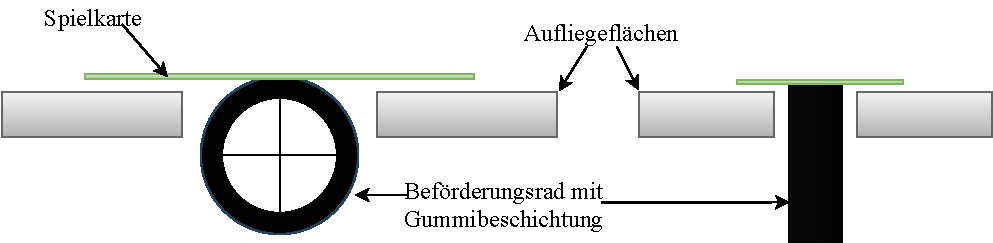
\includegraphics[scale=0.5,page=1]{fig/mech/RundesAusgaberad-Page-1}
    \caption{Rundes Ausgaberad}
\end{figure}

    Die einfachste Möglichkeit dieses Rad zu entwerfen, wäre ein einfaches rundes Ausgaberad. Dieses Rad wäre mit einer Schicht umhüllt, welche die Reibung
        dem Rad und der Karte erhöht. Das runde Rad wäre einfach zu fertigen und würde somit wenig kosten und nur einen geringen Zeitaufwand haben. Jedoch
        ist das Rad in der Lage mehr als nur eine Karte mit sich mitzuziehen, da es durchgehen Kontakt mit der Spielkartenoberfläche hat, dies hätte zur
        Folge, das mehrere Spielkarten zugleich weiterbefördert werden.
\begin{itemize}
    \item \textbf{Eliptisches Ausgaberad}
\end{itemize}

\begin{figure}[H]
    \centering
    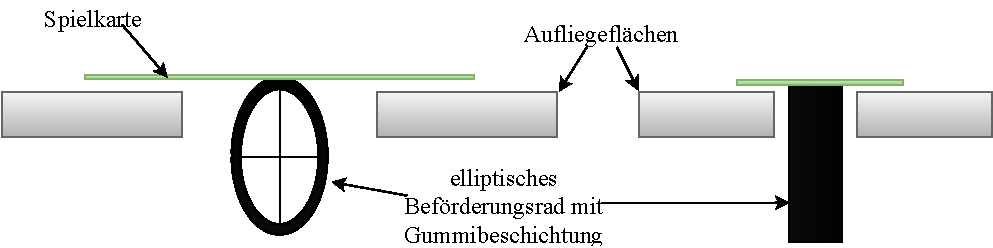
\includegraphics[scale=0.5,page=1]{fig/mech/ElliptischesAusgaberad}
    \caption{Eliptisches Ausgaberad}
\end{figure}


        Ein elliptisches Ausgaberad wäre das nächste Konzept, dieses Rad wird auch wie beim ersten Rad mit einem Motor verbunden um somit Karten zu befördern.
        Durch die elliptische Form des Rades herrscht kein durchgehender Kontakt mit der Oberfläche der Spilkarte, aus diesem Grund ist die Chance das mehrere
        Karten zugleich befördert werden minimiert. Jedoch setzt dies auch einen Motor vorraus der in kurzer Zeit ein hohes Drehmoment entwickelt, da die
        Karten schlagartig befördert werden. Das elliptische Rad würde in der Produktion auch mehr Kosten verursachen und wäre Zeitintesiver in der Hertellung. \\

\begin{itemize}
    \item \textbf{Vergleich der Ausgaberäder}
\end{itemize}

Da das primäre Ziel unserer Arbeit das perfekte Mischen der Spielkarten ist, wäre es besser das elliptische Ausgaberad in betracht zu ziehen. Die Kosten
 die durch die aufwendigere Herstellung entstehen wären überschaulich und somit wäre es nur profitabel dieses Konzept zu wählen. Durch die Tatsache das das elliptische Rad
das Kartendeck nur jede halbe umdrehung berrührt und nicht konstant, muss ein Motor für die Räder einegesetzt werden der sich schnell genug dreht um eine Karte mit einer berührung
des Rades "herauszuschießen". Dies würde aber keine zusätzlichen Kosten verursachen. Aus diesen Gründen fällt die Wahl auf das \textbf{elliptisches Ausgaberad}. \\

\subsection{Klemmmechanissmen}
Um beim Ausgeben und beim Weiterbefördern der Karten die Chance zu minimieren das mehrere Karten auf einmal weiterbefördert werden, wird ein
Klemmmechanissmus benutzt, dieser sorgt dafür das die Karten von außen Geklemmt werden, und somit nur die unterste Karte durch das Drehen des
Ausgaberades weiterbefördert wird.

\begin{itemize}
    \item \textbf{Primitiver Klemmmechanissmus}
\end{itemize}

\begin{figure}[H]
    \centering
    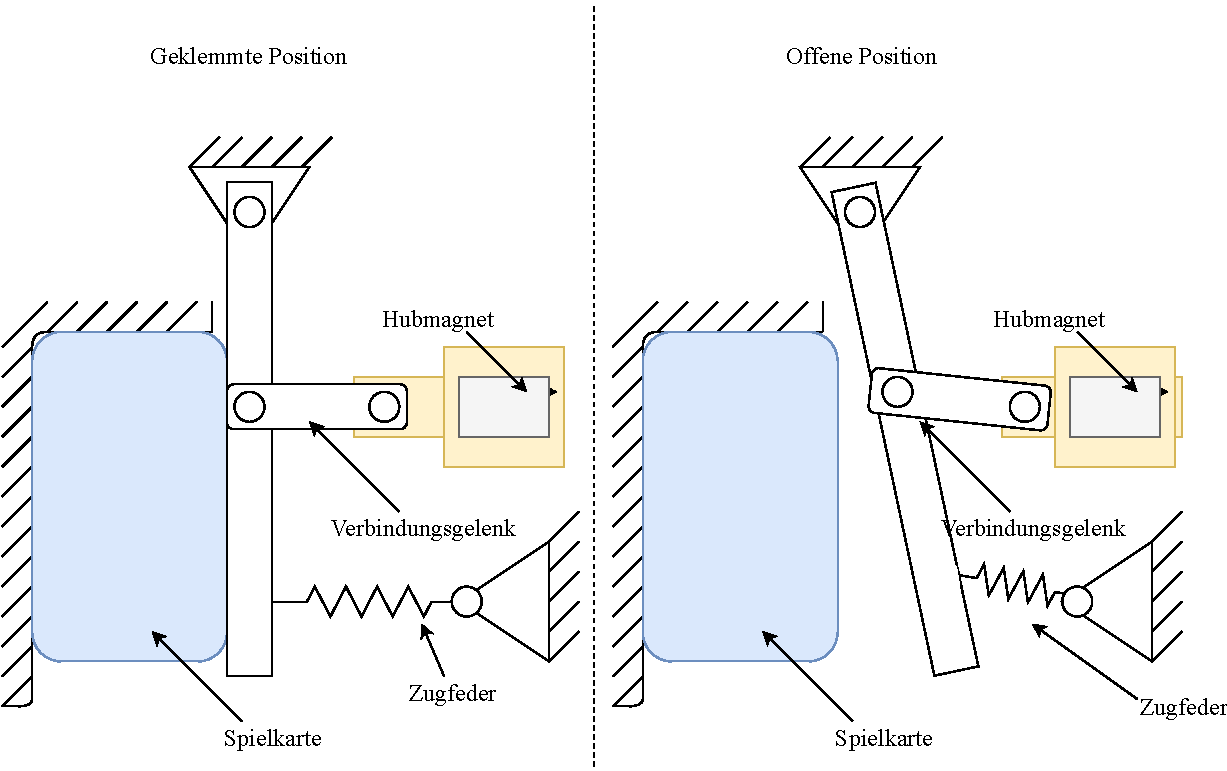
\includegraphics[scale=0.5,page=1]{fig/mech/Klemmmechanissmus1}
    \caption{Primitiver Klemmmechanissmus}
\end{figure}

Dieser Klemmmechanismus ist der primitivste und einfachste, dadurch aber auch der billigste. Die Karten werden auf der einen Seite an eine feste Wand gedrückt
auf der anderen Seite werden sie durch ein bewegliches Gelenk fixiert. Dieses Gelenk wrid durch das einschalten des Hubmagneten in die geschlossene Position bewegt,
soll das Gelenk wieder öffnen, so wird der Hubmagnet ausgeschalten und ein Zugfeder zieht das Gelenk wieder in seine Ausgangsposition zurück.

\begin{itemize}
    \item \textbf{Komplexer Klemmmechanissmus}
\end{itemize}

\begin{figure}[H]
    \centering
    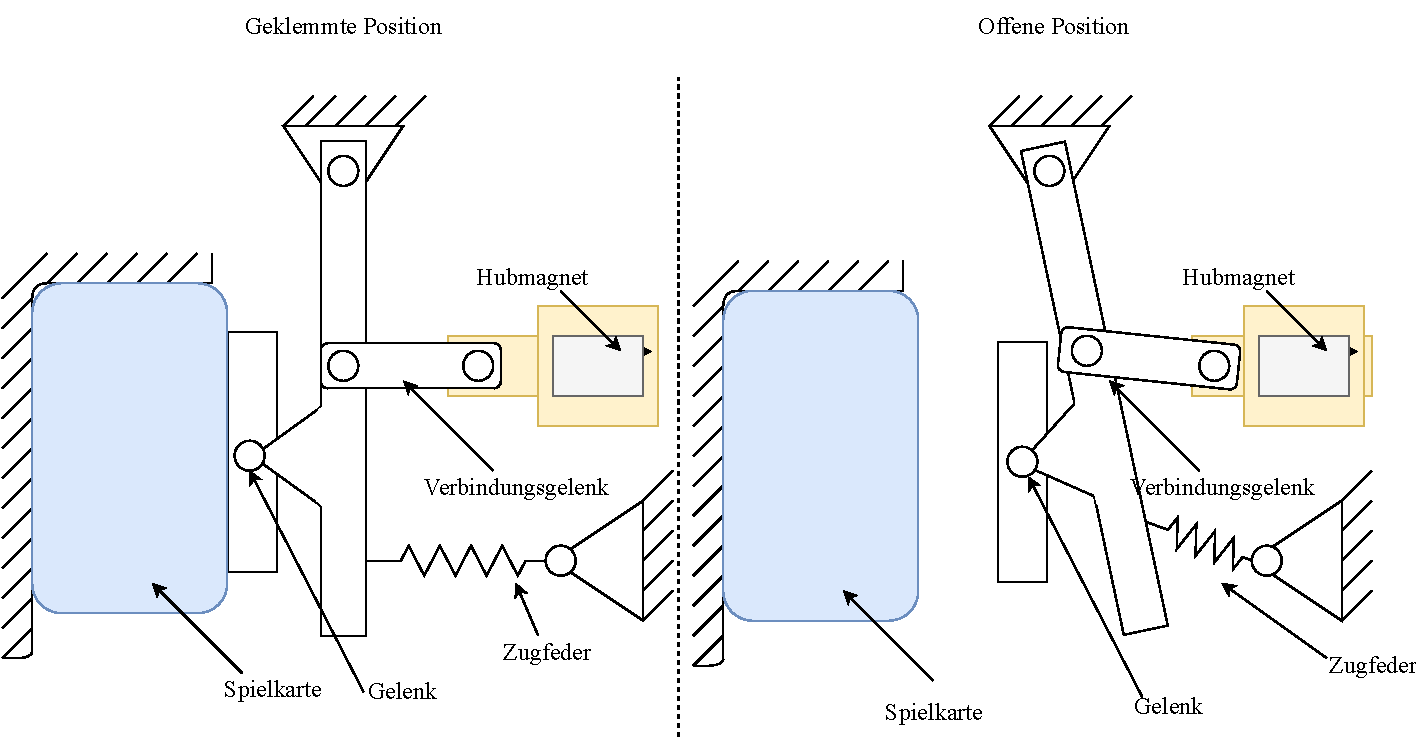
\includegraphics[scale=0.5,page=1]{fig/mech/Klemmmechanissmus2}
    \caption{Komplexer Klemmmechanissmus}
\end{figure}

Bei diesem Mechanissmus werden die Karten auf der einen Seite durch eine feste Wand geklemmt, auf der anderen werden sie durch ein Gelenk geklemmt, dieses Gelenk
ist beweglich und gleicht somit verschidene Kartengrößen aus. Um das Gelenk dieses Konzeptes zu schliesen wird ein Hubmagnet benötigt, wird dieser eingeschalten
so schließt das Gelenk und passt sich der Kartengröße an. Soll es wieder geöffent werden, so wird der Hubmagnet ausgeschaltet und eine Zugfeder bringt den Mechanissmus wieder in den
Grundzustand. Dieses Konzept ist aufwendiger zu realisieren wie das erste, jedoch kann es verschiedene Kartengrößen klemmen und gleicht sich den Karten an. Das Konzept ist
dafür aber auch aufwendiger in der Produktion.

\begin{itemize}
    \item \textbf{Gummi Klemmmechanissmus}
\end{itemize}

\begin{figure}[H]
    \centering
    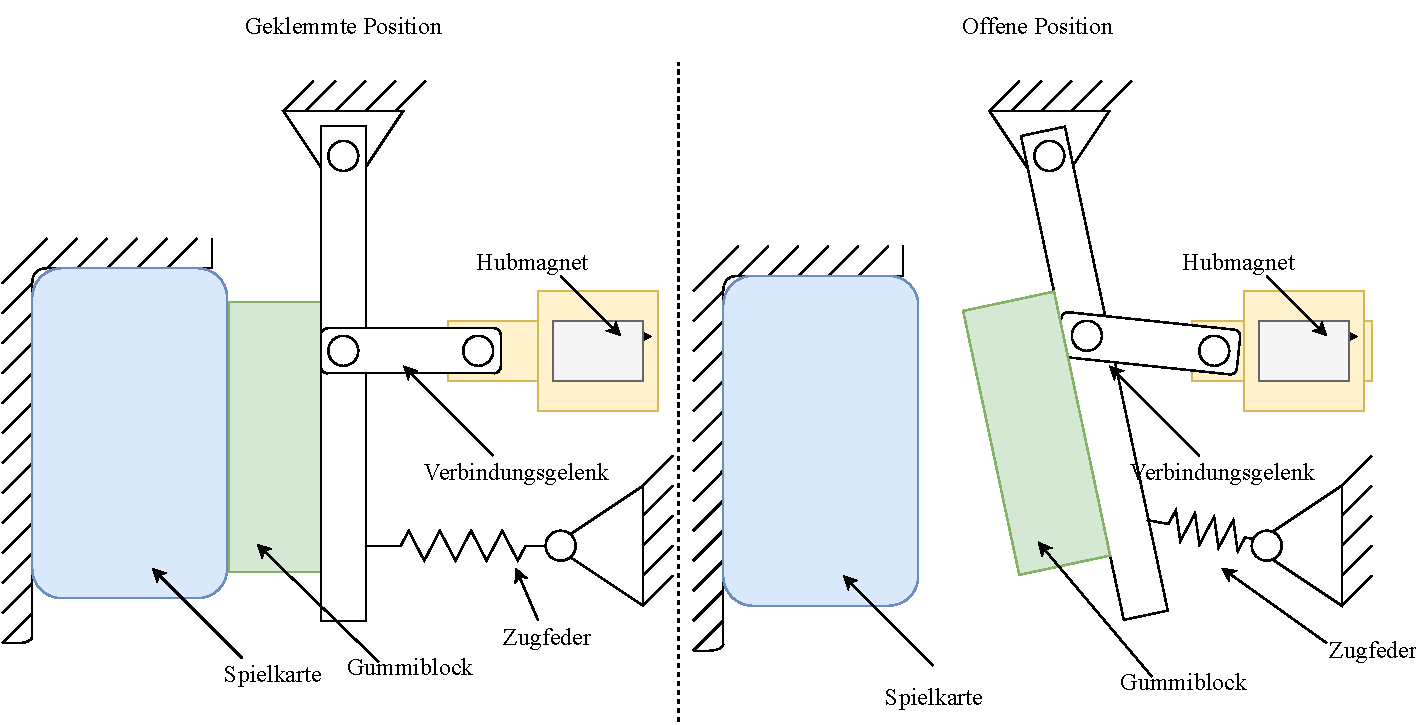
\includegraphics[scale=0.5,page=1]{fig/mech/Klemmmechanissmus3}
    \caption{Gummi Klemmmechanissmus}
\end{figure}

Der letzte Mechanissmus ist ufnktionsmäsig gleich wie der primitive Klemmmecahnissmus, der einzige Unterschied besteht aus dem
Gummiähnlichen Block der auf der Klemmfläche sitzt. Dieser soll sich den Karten anpassen und sorgt dafür das alle Karten gleichmäßig
 geklemmt werden, auch erhöht es die Reibung zwischen den Karten und der Klemmoberfläche. Dieses Konzept wäre in der  Herstellung verglichsweise
eifnach zu realisieren und dadurch auch billig in der Herstellung.


\begin{itemize}
    \item \textbf{Vergleich der Klemmmechanissmen}
\end{itemize}

Da alle Mechanissmen die gleiche Anzahl an Bateile erfordern, spielt der Preis bei dieser Auswahl keine große Rolle. Aus diesem Grund
sind die Kriterien Funktionalität und Aufwendigkeit in der Produktion. Der erst Mechanissmus wäre der einfachste in der Produktion, jedoch
hat er durch sein nicht anpassungsfähiges Klemmgelenk Probleme mit verschiedenen Kartengrößen, aus diesem Grund fällt er bei diesem Auswahlverfahren durch.
Der zweite Mechanissmus wäre der komplexe Klemmmechanissmus, dieser würde sich zwar verschiedenen Kartengrößen anpassen, wäre aber etwas aufwendiger in der
Produktion und ist somit auch nicht die bevorzugte Wahl. Der letzte Klemmechanissmus der einen gummiartigen Block auf der Klemmfläche hat, wäre einfach in der
Produktion und würde sich auch bei verschiedenen Kartengrößen anpassen, aus diesem Grund  fätt die wahl auf den Gummi Klemmmechanissmus.

\subsection{Seperation der Karten}
Da bei "Variante 3 - Lagerrad mit Saugnäpfe" Saugnäpfe mit Unterdruckprinzip in Verwendung kommen würden, liegt das Problem vor,
dass die Karten aneinander haften, dieses Problem entsteht durch den Unterdruck der beim Aufpressen des Saugnapfes entsteht.
Um zu garantieren das nur eine Karten in das Lager befördert wir oder ausgegeben wird, müssen diese aneinander
haftende Karten getrennt werden.

\begin{itemize}
    \item \textbf{Selbständiges Loslösen der Karten}
\end{itemize}

Die billigste und primitivste Möglichkeit die Karten zu separieren wäre abzuwarten bis alle Karten sich durch die Schwerkraft
von der eigentlich angesaugten Karte getrennt haben. Jedoch zeigten Versuche die durchgeführt wurden dass dies zu lange
dauern würde und das Spielerlebniss somit beeinflussen würde.

% Please add the following required packages to your document preamble:
% \usepackage{multirow}
\begin{table}[H]
    \centering
\scalebox{0.8}{
    \begin{tabular}{|c|c|c|c|c|c|c|c|}
        \hline
        \textbf{}                         & \multicolumn{7}{c|}{\textbf{Sekunden}}                                                                  \\ \hline
        \multirow{21}{*}{\textbf{Karten}} &    & 1. Durchgang & 2. Durchgang & 3. Durchgang & 4. Durchgang & 5. Durchgang        & Mittelwert       \\ \cline{2-8}
        & 20 & 9.69         & 9.32         & 8.92         & 8.54         & 4.53                & 8.2              \\ \cline{2-8}
        & 19 & 9.1          & 9.97         & 13.82        & 6.71         & 7.75                & 9.47             \\ \cline{2-8}
        & 18 & 15.39        & 8.93         & 6.51         & 13.05        & 15.25               & 11.826           \\ \cline{2-8}
        & 17 & 6.45         & 6.67         & 6.16         & 8.06         & 6.97                & 6.862            \\ \cline{2-8}
        & 16 & 10.76        & 6.52         & 10.62        & 11.37        & 6.97                & 9.248            \\ \cline{2-8}
        & 15 & 12.81        & 6.45         & 16.22        & 8.74         & 4.7                 & 9.784            \\ \cline{2-8}
        & 14 & 3.46         & 9.78         & 11.72        & 5.85         & 6.39                & 7.44             \\ \cline{2-8}
        & 13 & 4.85         & 8.18         & 10.77        & 10.5         & 3.43                & 7.546            \\ \cline{2-8}
        & 12 & 15.1         & 5.37         & 12.36        & 8.54         & 12.31               & 10.736           \\ \cline{2-8}
        & 11 & 15.83        & 6.32         & 5.58         & 5.08         & 1.12                & 6.786            \\ \cline{2-8}
        & 10 & 7.14         & 8.4          & 11.21        & 12.76        & 4.43                & 8.788            \\ \cline{2-8}
        & 9  & 7.48         & 6.24         & 11.87        & 4.32         & 6.36                & 7.254            \\ \cline{2-8}
        & 8  & 4.68         & 5.65         & 8.61         & 5.2          & 4.41                & 5.71             \\ \cline{2-8}
        & 7  & 9.73         & 8.29         & 9.13         & 5.35         & 11.2                & 8.74             \\ \cline{2-8}
        & 6  & 5.41         & 5.16         & 8.05         & 4.98         & 9.73                & 6.666            \\ \cline{2-8}
        & 5  & 6.06         & 4.81         & 7.8          & 4.73         & 7.19                & 6.118            \\ \cline{2-8}
        & 4  & 4.86         & 9.87         & 7.74         & 9.51         & 7.4                 & 7.876            \\ \cline{2-8}
        & 3  & 4.54         & 11.31        & 4.31         & 6.74         & 10.82               & 7.544            \\ \cline{2-8}
        & 2  & 4.83         & 2.19         & 4.13         & 3.78         & 5.71                & 4.128            \\ \cline{2-8}
        &    &              &              &              &              & \multicolumn{2}{c|}{Mittelwert: 7.932} \\ \hline
    \end{tabular}}
    \caption{Tabelle Haftzeit der Karten}
    \label{tab:my-table}
\end{table}

\begin{figure}[H]
    \centering
    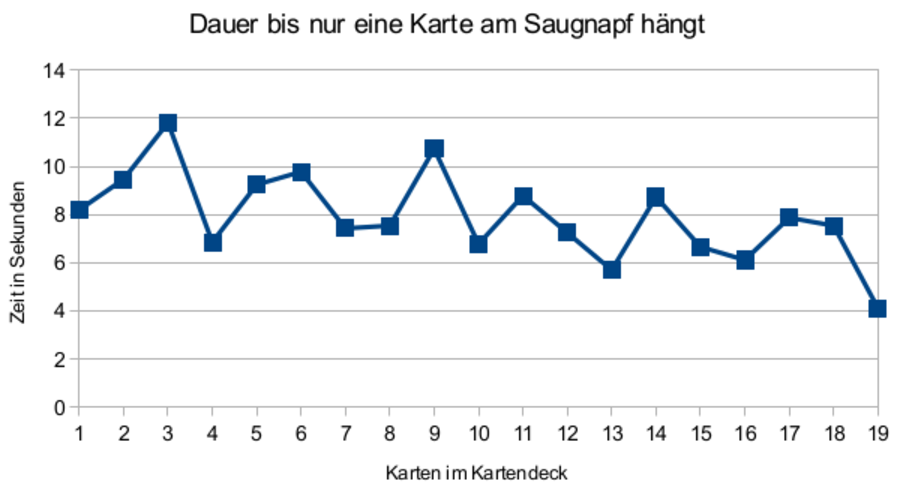
\includegraphics[scale=1,page=1]{fig/mech/Haftzeit}
    \caption{Diagramm Haftzeit der Karten}
\end{figure}

Wie man in Tabelle 1.1 und in Abbildung 1.9 erkennen kann dauert es im Durchschnitt 7,932 sekunden bis sich nur mehr die
eigentlich angesaugte Karte in der Luft befindet. der Versuch wurde mit 1Kg Ansaugdruck durchgeführt. Es gab insgesamt
5 Durchgänge, auch wurden alle Möglichkeiten der Kartenanzahlen im Kartendeck berücksichtigt, so saugte der Saugnapf
bei der ersten Durchgangsreihe die erste Karte an, die auf 19 anderen Karten liegt , bis hin zu einem Saugnapf der
eine Karte ansaugt die nur auf einer einzelnen anderen Karte liegt.

\textbf{Vorteile:}
\begin{itemize}
    \item billig
    \item keine zusätzlichen Bauteile benötigt
\end{itemize}
\textbf{Nachteile:}
\begin{itemize}
    \item lange Wartezeit
    \item unzuverlässig
\end{itemize}

\begin{itemize}
    \item \textbf{Rütteln}
\end{itemize}

Ein weiteres Konzept um die angesaugte Karten von den anderen zu Trennen wäre die Karten minimal zu rütteln.
Da die angesaugt Karte viel stärken an dem Saugnapf haftet als die Karten, die nur an der angesaugten Karten haften,
könnte der Hubmagnet oder der ansaugmechanissmus leicht gerüttelt werden, so würden die anderen Karten schneller den
Unterdruck untereinander verlieren und sich somit schon in kurzer Zeit separieren lassen. Jedoch müsste für dieses Konzept
ein Mechanissmus entwickelt und produziert werden der nur einen ausgewählten Berreich rüttelt, dies wäre mit weiteren Bauteilkosten und
Aufwand verbunden.

\textbf{Vorteile:}
\begin{itemize}
    \item zuverlässig
\end{itemize}
\textbf{Nachteile:}
\begin{itemize}
    \item teurer
    \item zusätzliche Bauteile
    \item zusätzliche Größe
\end{itemize}


\begin{itemize}
    \item \textbf{Abstreifbürsten}
\end{itemize}

Bei diesem Konzept sind Bürstenartige Abstreifvorrichtungen in der Kartenhalterung angebracht. Diese Bürsten sollen beim aufheben der
angesaugeten Karte die anderen Karten die mitgehebt wurden abstreifen. Dabei ist es wichtig, dass die Bürste den richtigen Widerstand aufbringt.
Ist der Widerstand zu hoch, wird auch die eigentlich angesaugt Karte mitabgestreift, ist er jedoch zu niedrig ist es möglich, dass die anderen Karten
die mitgehoben werden nicht abgestreift werden.

\textbf{Vorteile:}
\begin{itemize}
    \item zuverlässig
    \item billig
\end{itemize}
\textbf{Nachteile:}
\begin{itemize}
    \item Karten werden seitlich abgenützt
    \item komplizierter Einbau
\end{itemize}

\begin{figure}[H]
    \centering
    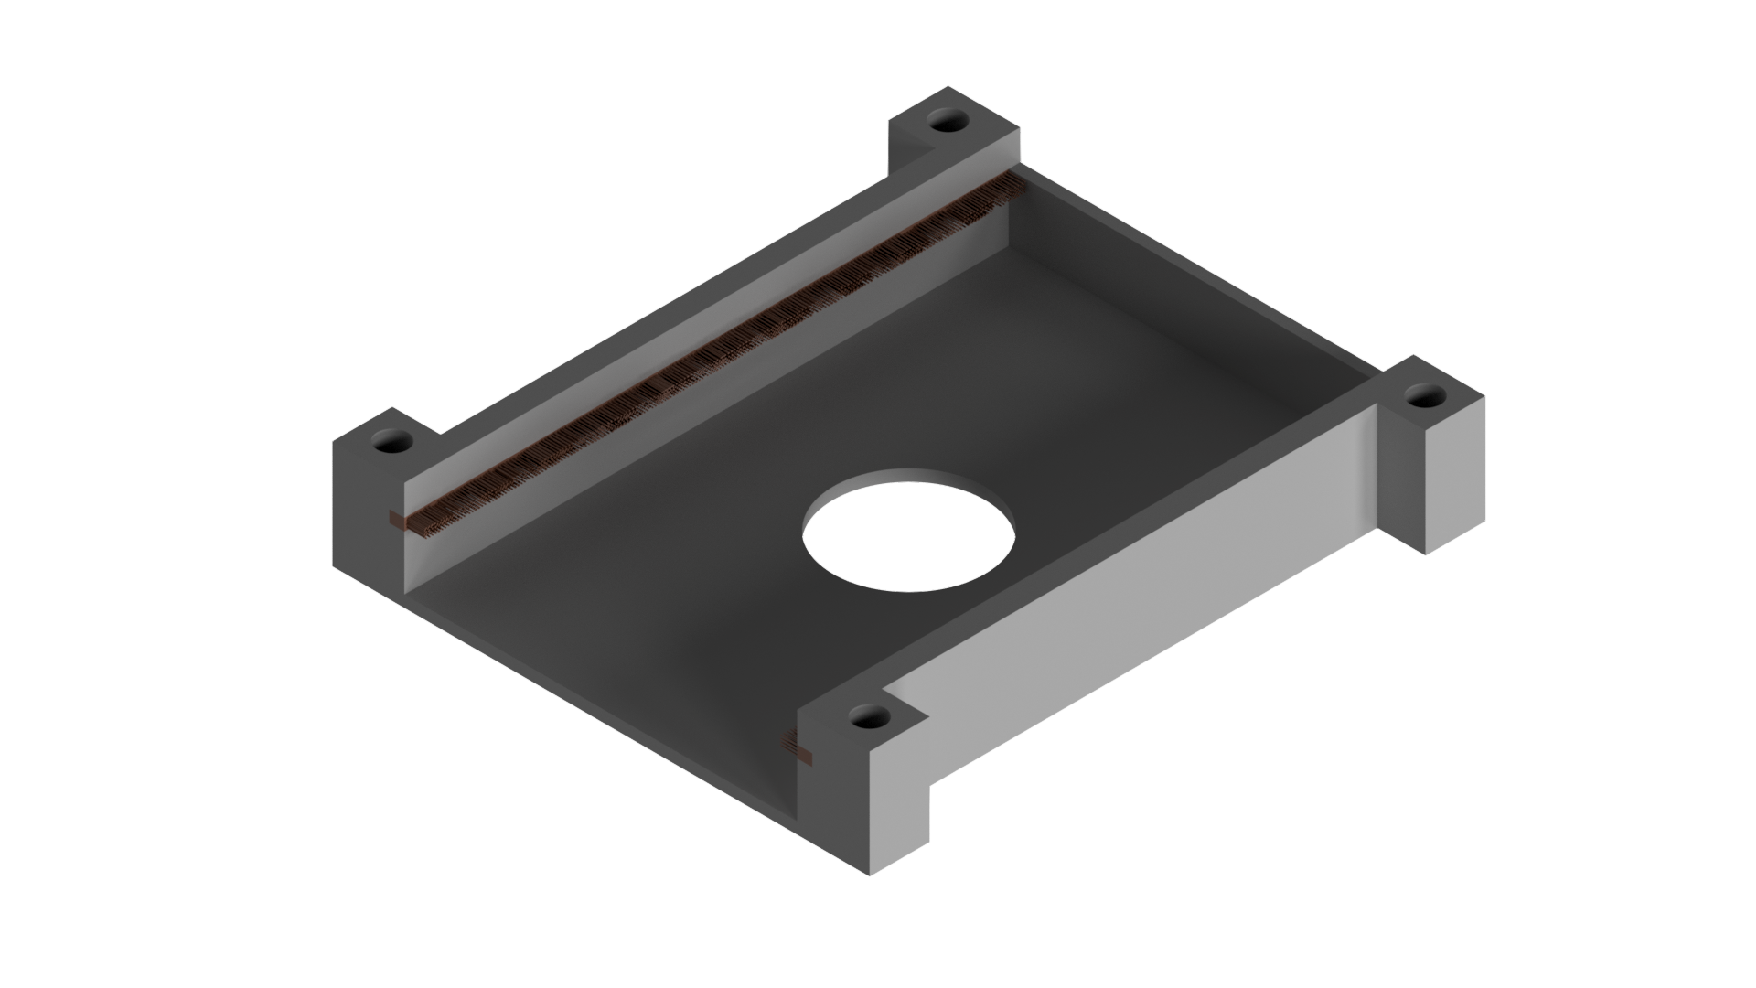
\includegraphics[scale=0.5,page=1]{fig/mech/AusgabeMitBuersten}
    \caption{Ausgabe mit Bürsten}
\end{figure}

\begin{itemize}
    \item \textbf{Gummiabsstreifer}
\end{itemize}

Dises Konzept funktioniert ähnlich wie das "Abstreifbürsten Konzept". Es besitzt seitlich Abstreifplatten die aus Gummi sind, diese
sollen der angesaugten Karte helfen die die migezogenen Karten abzustreifen. Wie beim vorherigen Konzept muss hierbei das Gummi auch so
dimensioniert werden, dass es einerseits nicht zu steif ist und die eigentlich angesaugt Karte abstreift, andererseits sollte es steif genug
sein um die Karten die mitgehoben werden abzustreifen. Man die Steifigkeit des Gummistreifens verändern, indem man die Breite der Einschnitte
erhöht oder vermindert.

\begin{figure}[H]
    \centering
    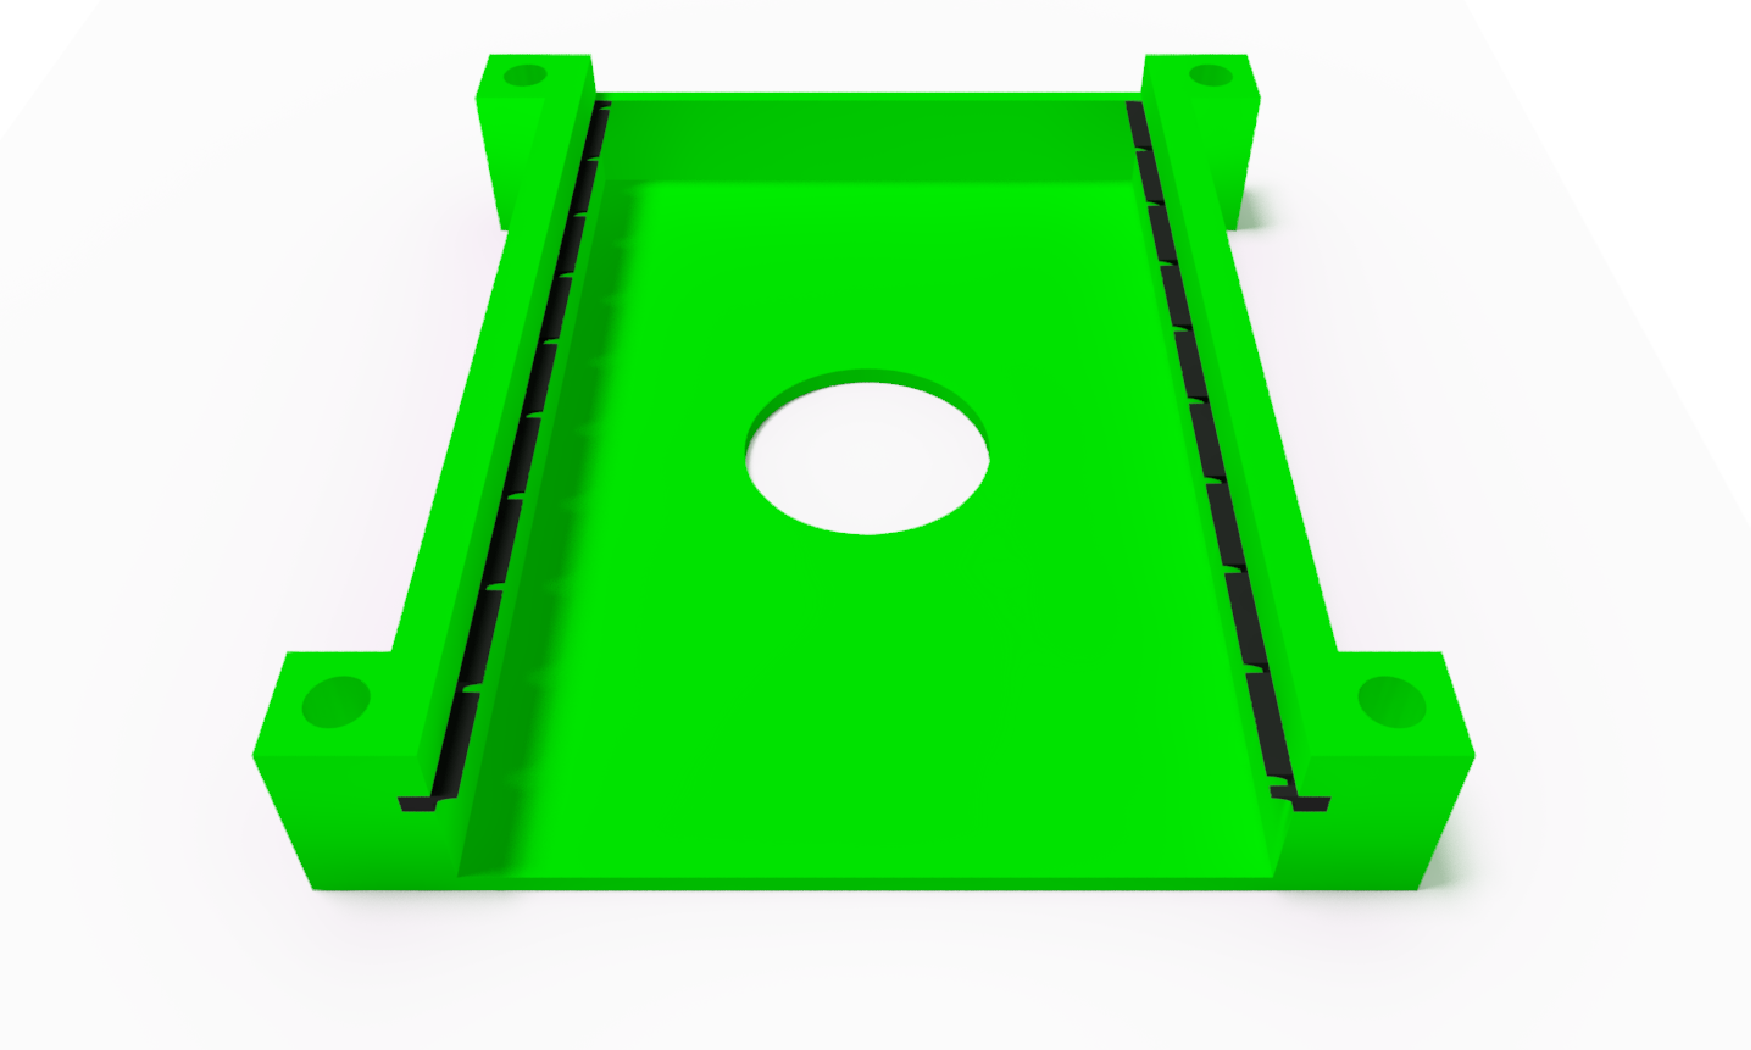
\includegraphics[scale=0.5,page=1]{fig/mech/AusgabeMitGummiabstreifer}
    \caption{Ausgabe mit Bürsten}
\end{figure}

\textbf{Vorteile:}
\begin{itemize}
    \item zuverlässig
    \item billig
\end{itemize}
\textbf{Nachteile:}
\begin{itemize}
    \item Gummi wird spröde
\end{itemize}

\subsection{Saugmechanismus}

Da bei der 3. Variante, Lagerrad mit Saugnäpfe, Saugnäpfe zum Einsatz kommen, muss entschieden werden, welche Saugnäpfe angewand werden.

\begin{itemize}
    \item \textbf{einfacher unterdruck Saugnapf}
\end{itemize}
Die erste Möglichkeit wäre einen einfachen Saugnnapf zu nehemen, der durch anpressen an einer Oberfläche einen Unterdruck erzeugt und somit Haftet. Ein Vorteil dieses Saugnapfes ist es, das es kostengünstig ist und keine weiteren Bauteile benötigt, sowie die
unkomplizierte Befestigung an dem Hubmagneten über ein Gewinde.
Jedoch muss dieser Saugnapf mit einer gewissen Kraft auf das Kartendeck gepresst werden, um einen Unterdruck erzeugen zu können, die kann dazu führen, dass die Karten untereinander auch ein Vakuum erzeugen und somit mehr als eine Karte vom Saugnapf
hochgehoben wird. Ein weiterer Nachteil wäre, das die Karte nicht steuerbar abwerfbar ist, da sie erst abfällt, wenn der Unterdruck verschwindet, dies kann zu unerwarteteten Wartezeiten führen. Wenn der Ansaugdruck durch den Hubagneten nicht erreicht wird, kann
es auch dazu führen, dass keine Karte angesaugt wird, dies kann die Wartezeiten wiederum verlängern und somit den Spielablauf stören.

\textbf{Vorteile:}
\begin{itemize}
    \item Billig
    \item unkomplizierter Einbau
\end{itemize}
\textbf{Nachteile:}
\begin{itemize}
    \item unzuverlässig
\end{itemize}

\begin{itemize}
    \item \textbf{vakuum Saugnapf}
\end{itemize}
Eine andere Möglichkeit wäre ein vakuum Saugnapf, dieser erzeugt seinen Unterdruck über eine Vakuumpumpe und kann somit gesteuert werden. Der Vorteil dieses Saugnapfes ist es, das die Karten zu einer gewünschten Zeit abgeworfen werden können, da man den
Unterdruck des Saugnapfes durch die Pumpe steuern kann. Ein anderer Vorteil ist, dass der Hubmagnet keine hohe Kraft aufweisen muss, da der Saugnapf nicht mehr auf die Karten aufpressen muss, dies würde auch das Problem das mehrere Karten auf einmal
aufgehoben werden lösen. Der Nachteil dieser Möglichkeit wäre jedoch der erhöte Preis des Saugnapfes sowie die zusätzlichen Bauteile, wie zum Beispiel die Pumpe und die Valve. Außerdem ist der Einbau des Saugnapfes etwas komlizierter, da ein Luftdruckschlauch
zum Saugnapf geführt werden muss.

\textbf{Vorteile:}
\begin{itemize}
    \item Zuverlässig
    \item Unterdruck ist kontrollierbar
\end{itemize}
\textbf{Nachteile:}
\begin{itemize}
    \item mehr Bauteile
    \item teuer
    \item komplizierter Einbau
\end{itemize}

\begin{itemize}
    \item \textbf{Vergleich der Saunäpfe}
\end{itemize}

Beide Saugnäpfe würden ihre idividuelle Vorteile besitzen. Da wir zum einen ein begrenztes Budget habe wäre der einfache unterdruck Saugnapf für uns attrektiv, zum anderen wäre der vakuum Saugnapf druch seine zuerlässigkeit vom Vorteil.
Da der ausgewählt Hubmagnet jedoch nicht in der Lage ist den erforderlichen Ansaugdruck zu erreichen, und das kontrollierte abwerfen der Karten massgeblich für ie Funktion der Maschine ist, fällt unsere Auswahl auf den \textbf{vakuum Saugnapf}.
\subsection{Endauswahl der Varianten}

\textbf{\large{Gegenüberstellung der Varianten}}

\begin{table}[H]
\centering
\scalebox{0.8}{
    \begin{tabular}{|c|c|c|ll}
        \cline{1-3}
        \textbf{Variante}             & \textbf{Vorteile}                                                                & \textbf{Nachteile}                                                                                    &  &  \\ \cline{1-3}
        1 - Linearachsen              & \begin{tabular}[c]{@{}c@{}}schnelles Mischen\\ wenige Fehlerquellen\end{tabular} & \begin{tabular}[c]{@{}c@{}}teuer\\ großer Aufbau\\ instabil\end{tabular}                              &  &  \\ \cline{1-3}
        2 - Lagerrad mit Ausgaberäder & \begin{tabular}[c]{@{}c@{}}stabil\\ niedriger Aufbau\end{tabular}                & \begin{tabular}[c]{@{}c@{}}lange Gesamtgröße\\ viele Bewegliche Bauteile / Fehlerquellen\end{tabular} &  &  \\ \cline{1-3}
        3 - Lagerrad mit Saugnäpfe    & \begin{tabular}[c]{@{}c@{}}billig\\ wenig bewegliche Bauteile\end{tabular}       & hoher Aufbau                                                                                          &  &  \\ \cline{1-3}
    \end{tabular}}
    \caption{Vergleich der Varianten}
\end{table}

\textbf{\large{Begründung der Wahl}}\\
Alle drei Varianten wurden durchdacht und bieten ihre individuellen Vorteile. Durch den enormen Preis von
Variante 1 ist diese aber nicht für unser Projekt geeignet. Das optimale Konzept des Mischens wird am besten durch
Variante 3 realisiert, da diese die niedrigste Wahrscheinlichkeit aufweist, mehrere Karten aufeinmal in das Lager zu befördern.
Da Variante 3 im Vergleich zur Variante 2 weniger Bauteile besitzt, ist diese Variante sowohl Preislich ansprechender für uns
 sowie auch die Tatsache das Fehlerquellen durch bewegliche Bauteile minimiert werden. \\
Somit fällt die finale Wahl auf \textbf{Variante 3}.



\pagebreak
\section{Konstruktion}
\subsection{Konstruktion des Lagerrades}
Das Lagerrad soll durch das zufällige Rotieren das Mischen der Karten ermöglichen. Im Verlauf der Diplomarbeit wurde das Lagerrad mehrfach überarbeitet.
Die grundsätzliche Form dieses Rades besitzt ein virtel eines Hohlzylinders der in mehreren Fächern unterteilt ist. Die erste Version dieses Rades besaß 20 Unterteilungen.

\begin{figure}[H]
    \centering
    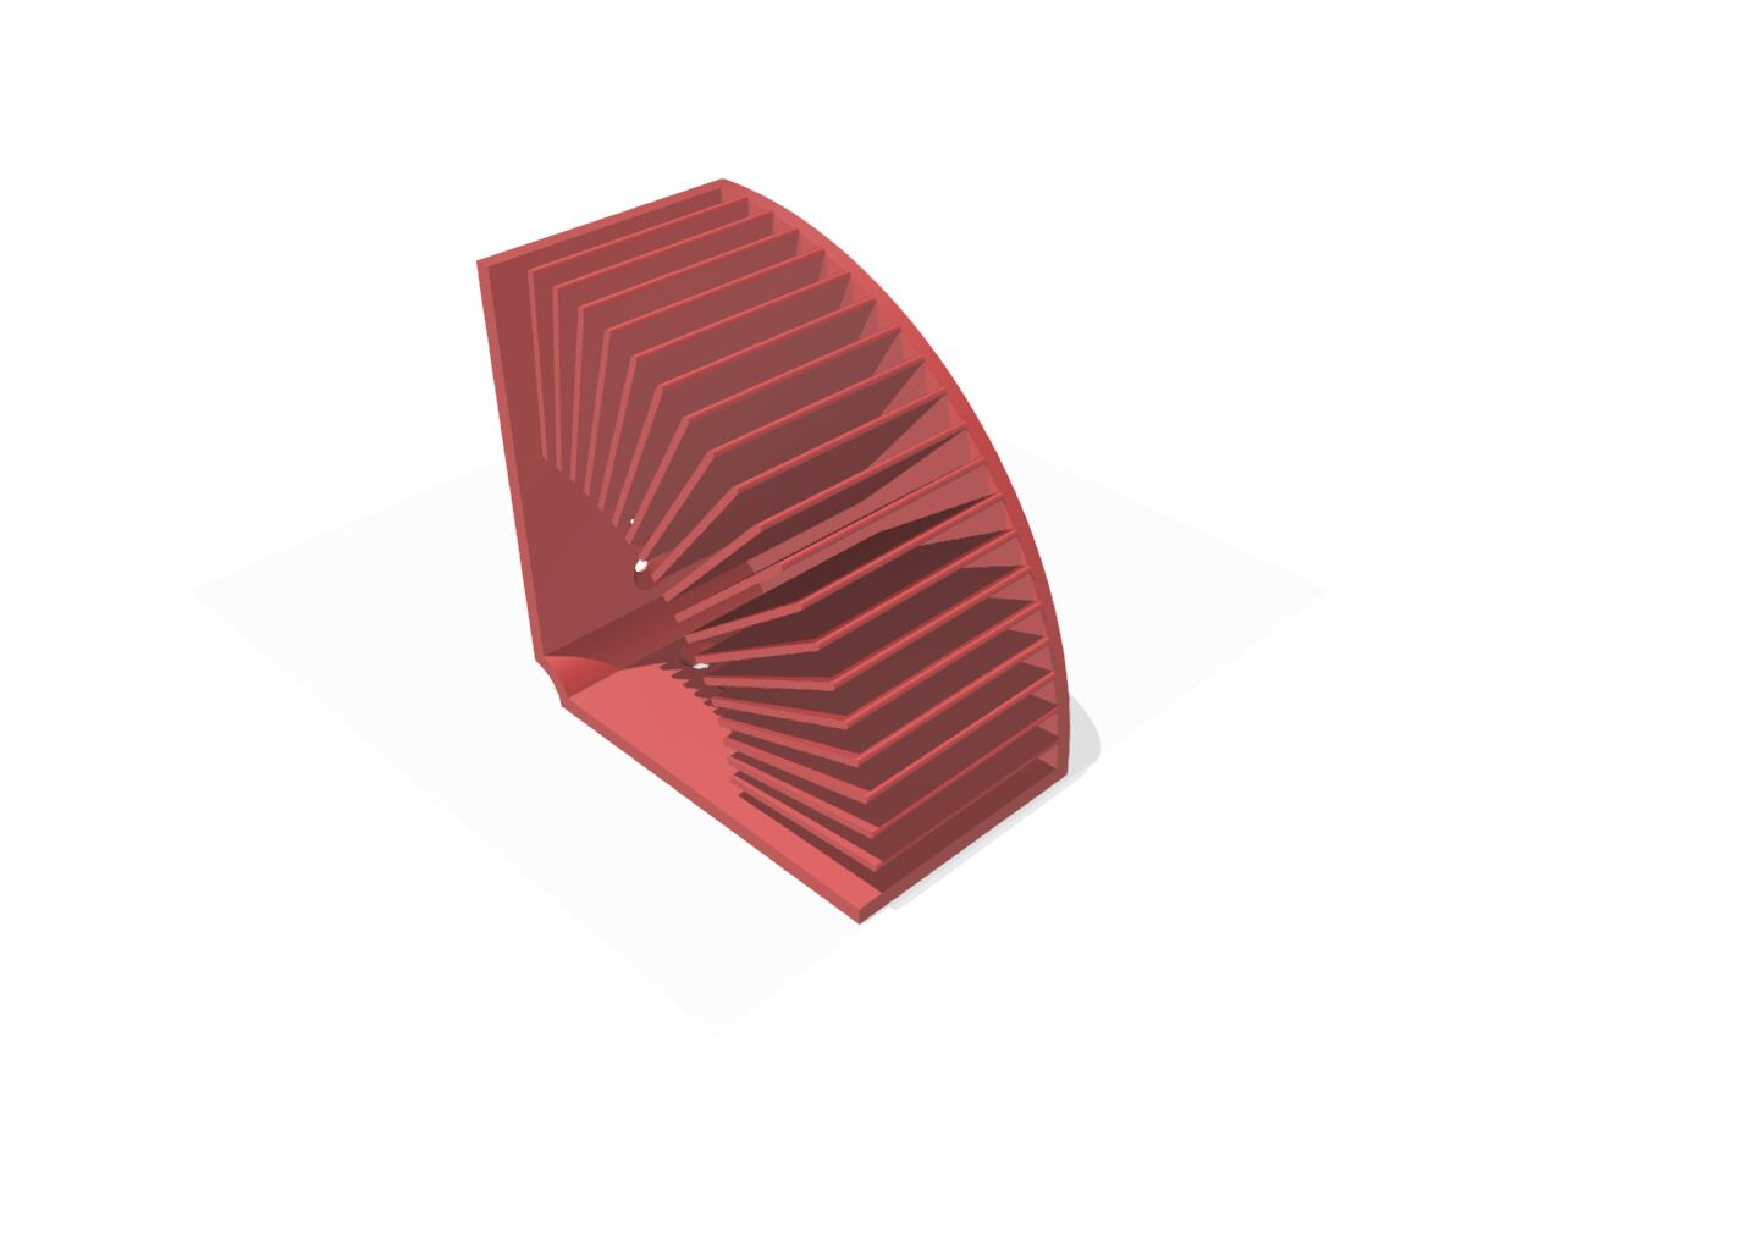
\includegraphics[scale=0.5,page=1]{fig/mech/LagerRad20F}
    \caption{Version 1: Lagerrad 20 Fächer (geöffnete Außenwand zur vereinfachten Ansicht)}
\end{figure}

In der oben angezeigen Grafik wurde die Außenwand entfernt um eine bessere Einsicht in das Bauteil zu bekommen.
Durch die 20 Unterteilungen muss der Schrittmotor genauere Positionen anfahren, außerdem wäre der Aufwand beim produzieren groß. Aus diesem Grund
entschieden wir uns die Unterteilungen zu minimieren, und kamen zu dem Entschluss, dass 4 Unterteilungen für ein optimales Mischen ausreichen. Diese Konstruktion
wurde nach einem Stecksystem entworfen, sodass man die einzelnen Teile herstellen kann und diese dannach zusammenstecken und verkleben kann.

\begin{figure}[H]
    \centering
    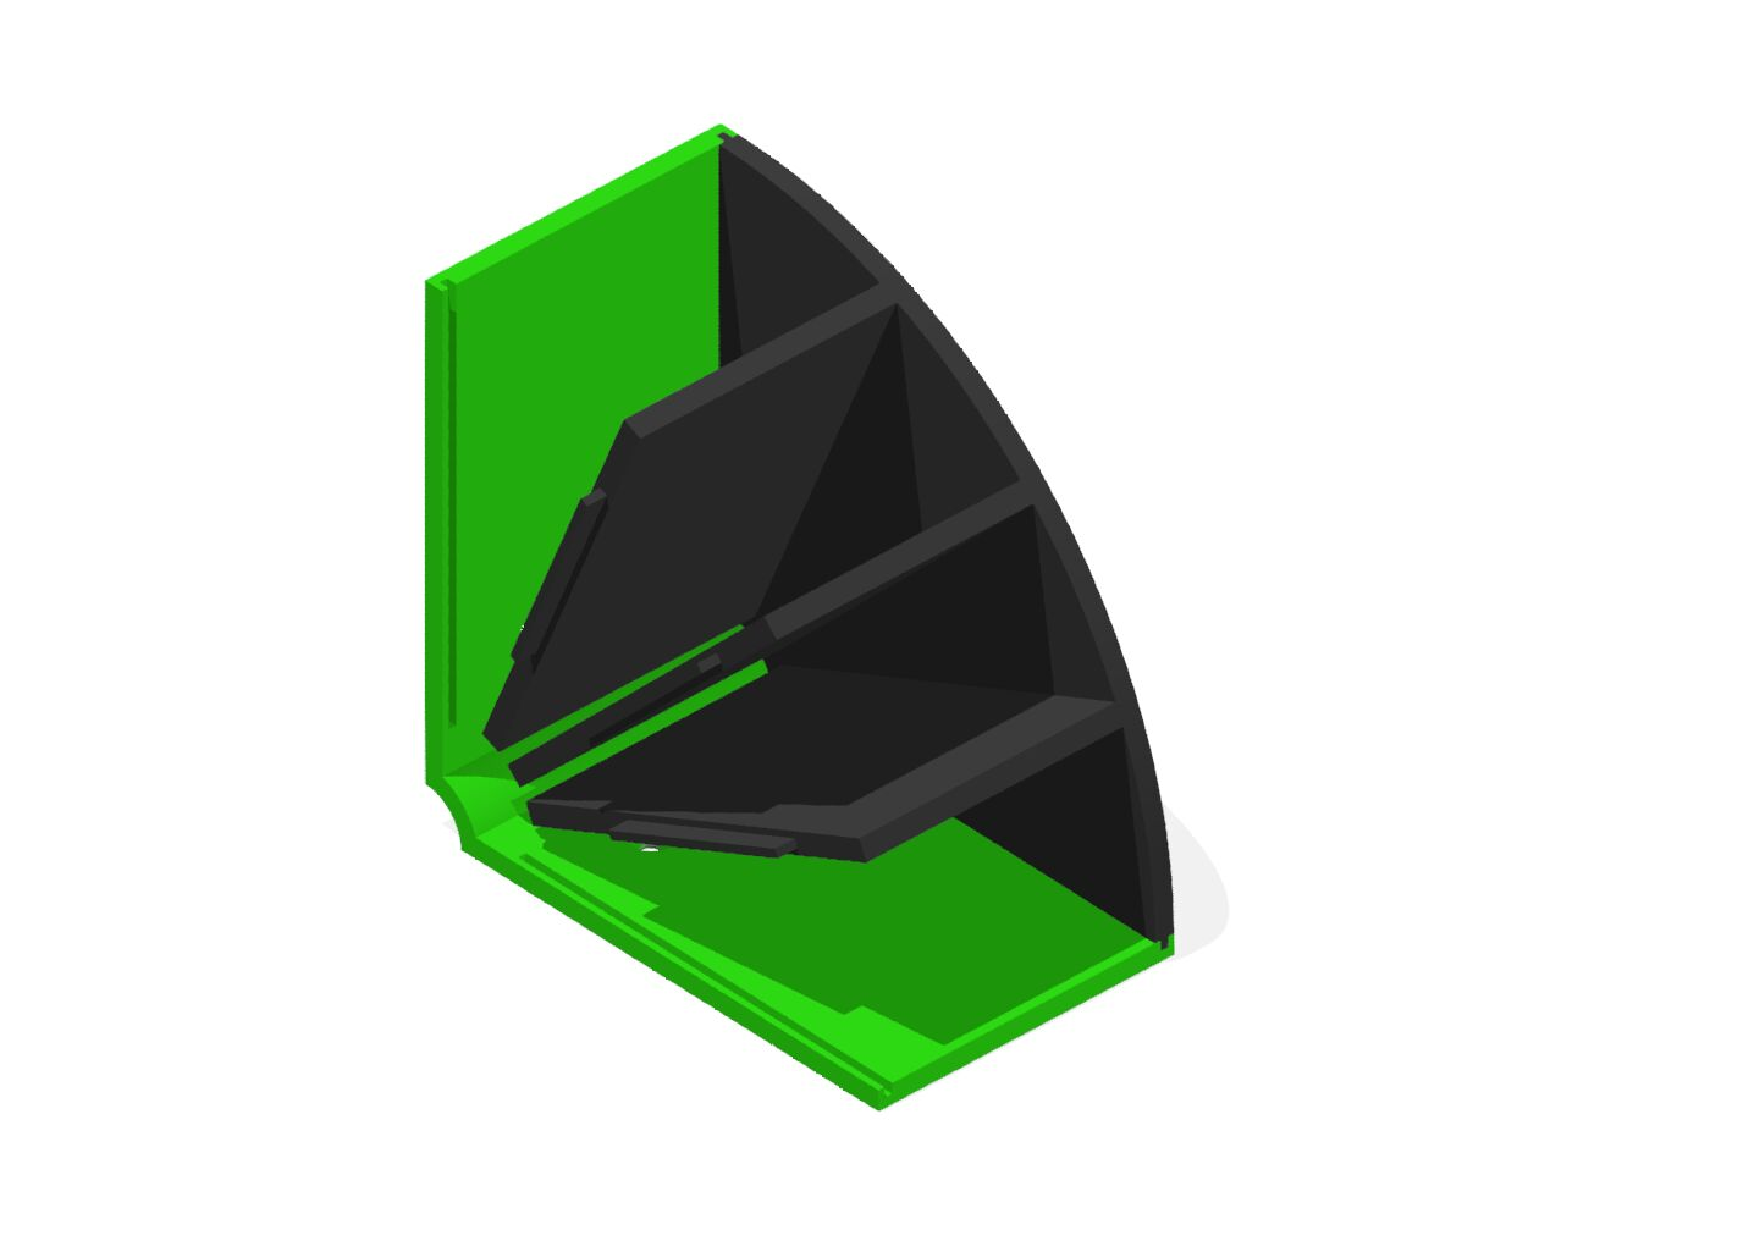
\includegraphics[scale=0.5,page=1]{fig/mech/LagerRad4F}
    \caption{Version 2: Lagerrad 4 Fächer (geöffnete Außenwand zur vereinfachten Ansicht)}
\end{figure}


Auch in der oben gezeigten Grafik wurde die Außenwand entfernt um das Bauteil besser zu veranschaulichen.
Das Lagerrad besteht aus mehreren Einzelteilen:

\subsubsection{Außenwände}
Die Außenwände wurden in der Form eines Teil eines Kreises konstruiert und geben somit die Fporm des Lagerrades vor. Sie besitzten jeweils 2 Laschen an der äußeren Seite, diese verboinden die Außenwände später mit den Seitenwänden es LAgerrades.
Außerdem besitzen sie jeweils 3 Ausfräsungen auf Ihrer Grundfläche, über die sie später mit den Trennplatten versteckt werden. Bei der Konstruktion der ausfräsungen ist dabei zu achten, dass etwas größer als benötigt gezeichnet werden, da bei der
Fertigungsart des 3D Druckens Innenbohrungen und Innenfräsungen durch die ungenauigkeit des Druckers kleiner gedruckt werden. Wie auch bei den Innenfräsungen müssen die Laschen auf der Außenseite etwas kleiner konstruiert werden, da diese woederum beim
drucken größer gedruckt werden als sie Ursprünglgich gezeichnet wurden.

\subsubsection{Seitenwände}
Diese Bauteile verbinden das Lagerrad mit der Lagerradhalterungsmodul. Sie besitzen auf der äußeren Seiter der Grundfläche
jeweils 2 Auskerbungen, über diese werden sie mit den Laschen der Außenwände verbunden. Um einen Durchgang für die Welle zu schaffen
schließen die Bauteile auf der unteren Seite nicht im rechten Winkel ab, sondern sind nach innen radial abgerundet.
Je Bauteil sind 2 Bohrungen vorhanden, über diese wir es mit der Lagerradhalterungsmodul verbunden.
Die Bohrungen sind als Senklochbohrungen ausgeführt, da somit die Schraube komplett in das Bauteil versenkt werden kann
 und das hineinrutschen der Karten in das Lagerrad nicht behindert wird.

\subsubsection{Trennplatte}
Um die einzelnen Lagerfächer zu unterteilen ist die Trennplatte konsturiert worden. Dieses Bauteil ist ein einfacher
Quader mit je 2 Laschen an den Außenseiten. Diese Laschen werden mit den Ausfräsungen der Außenplatte versteckt.
Hierbei ist wieder zu achten, das die Laschen kleiner konstruiert werden, da sie durch den 3D druck an größe zunehmen
werden.

\subsection{Konstruktion des Lagerradhalterungsmoduls}
Um das Moment der Welle effektiv von der Welle zum Rad übertragen wurde ein Lagerradhalterungsmodul entworfen. Dieses Modul wird
benötigt, da das Wellenmoment nicht effektiv an einem 3D gedruckten Bauteil angreifen kann, da das gedruckt PLA
die kontinuierlichen Richtungswechsel sowie das abrupte Bremsens des Motors in kombination mit der
Trägheit des Lagerrades nicht standhalten würde. Dieses Modul besteht aus folgenden Einzelteilen:

\subsubsection{L-Grundplatte}
Dieses Bauteil verbindet die Motorwelle sowie die Lagerwelle mit der Verbindungsplatte und somit auch mit dem Lagerrad, es
überträgt somit auch das Moment des Motors. Es besitzt je 4 Bohrungen mit Zylinderschrauben Senkungen über die sie mit
der Verbindungsplatte verbunden wird. Außerdem besitzt sie eine Bohrung mit einer Querbohrung. Über diese werden die
Wellen geführt und mit einer Schraube am Bauteil fixiert.
Dieses Bauteil wurde ürsprünglich aus Aluminium gefertig, durch Versuche mit einer 3D gedruckten L-Grundplatte zeigte
sich jedoch, dass diese sich genau so gut eignet und optisch ansprechender ist. Um nicht in konflikt mit dem Lagerrad
zu stehen hat das Bauteil jeweils 2 ausbuchtungen nahe der Welle.

\subsubsection{Verbindungsplatte}
Die Verbindungsplatte nimmt das von der L-Grundplatte aufgenommene Moment des Motors und überträgt es an das Lagerrad weiter.
Sie wurde als einfacher Aluminiumquader konstruiert und besitzt insgesamt 6 Bohrungen. Zwei Bohrungen sind auf der
Grundfläche des Bauteils und besitzten ein Gewinde. Diese verbinden Lagerradhalterungsmodul mit dem Lagerrad. Je 2
Bohrungen sitzen auf der Unterseite sowie auf der Oberseite der Verbindungsplatte und sind ebenfalls mit Gewinde
ausgeführt, durch diese Gewindebohrungen Verbinden das L-Bauteil mit der Verbindungsplatte.
Dieses Bauteil wurde aus Aluminium gefertig da es problematisch ist ein Gewinde in PLA zu schneiden, außerdem spielt
das zusätzliche Gewicht des Aluminiums bei diesem Modul nur eine geringe Rolle.

\subsubsection{Motorwelle}
Um das Moment vom Motor auf die L-Grundplatte zu übertragen wird die Motorwelle benötigt. Diese ist eine einfache Welle
mit einer Gewindebohrung am äußeren ende der Welle. Diese dient dazu, die Welle mit der L-Grundplatte zu verbinden.
Am anderen Ende ist die Welle über die Kupplung mit dem Motor verbunden.
Die Welle wurde an der Drehbank gefertigt und anschließend an der Fräsmaschine die Gewindebohrung gebohrt..

\subsubsection{Lagerwelle}
Die Lagerwelle unterscheidet sich von der Motorwelle lediglich durch ihre Länge. Sie wird einerseits mit der
L-Grundplatte verschraubt, auf der anderen Seite wird sie mit dem Zweiloch-Flanschlager auf der Vorderseite des Gehäuses über
2 Wurmscchrauben geklemmt.

\begin{figure}[H]
    \centering
    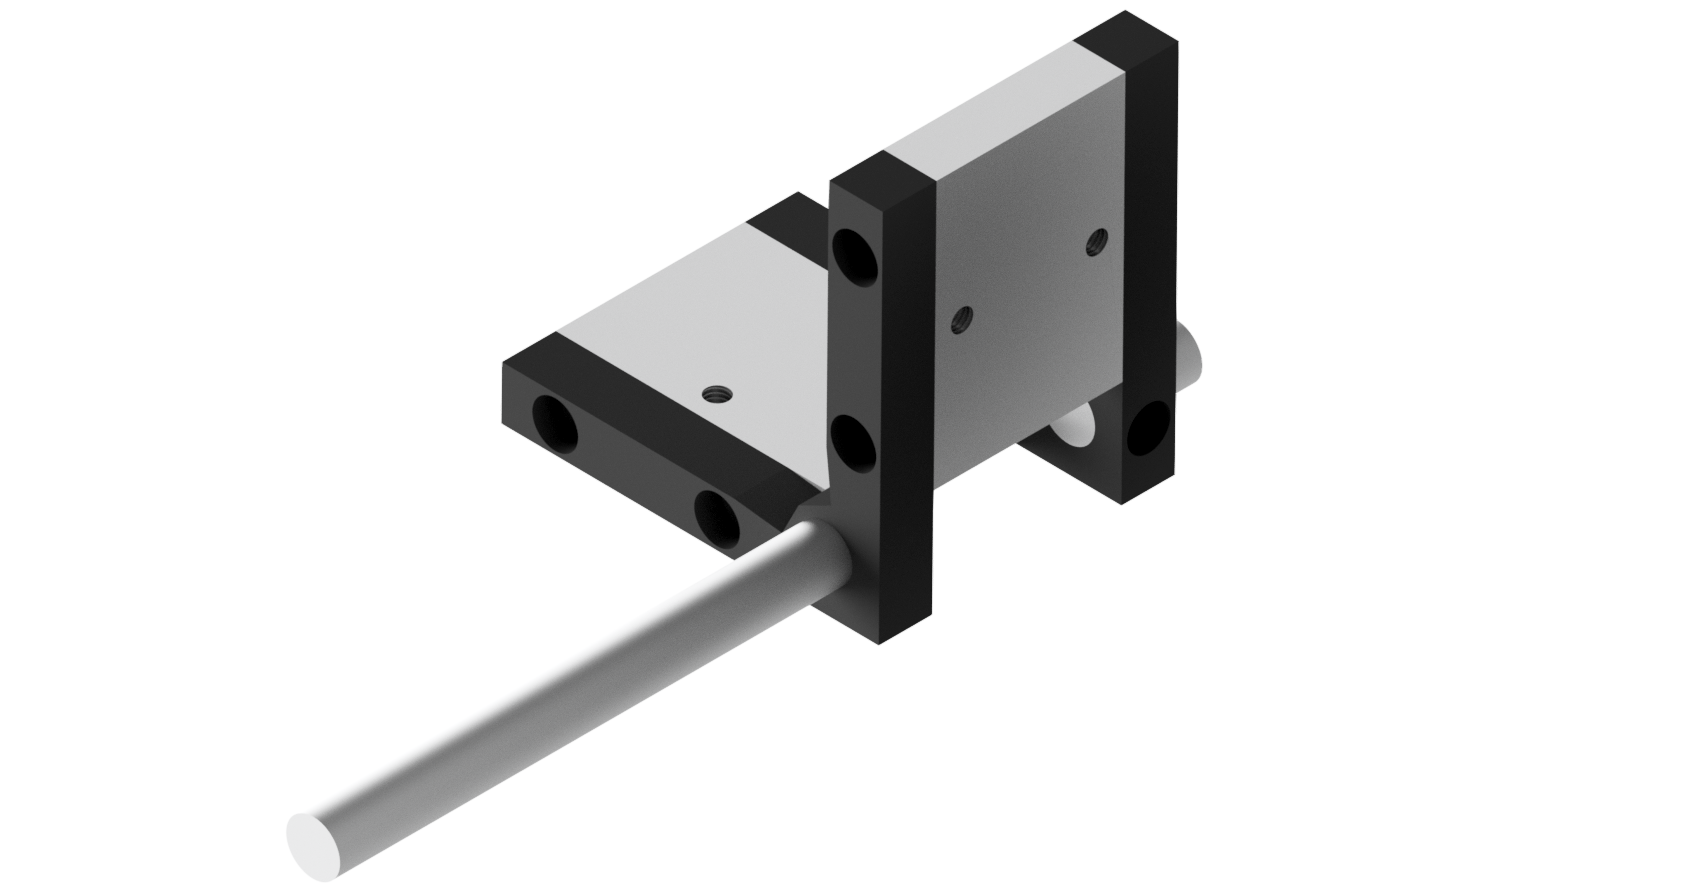
\includegraphics[scale=0.25,page=1]{fig/mech/LagerRadGruppekomplett}
    \caption{Lagerradhalterungsmodul}
\end{figure}

\subsection{Konstruktion der Motorhalterungsgruppe}

Die Motorhalerung hat den Zweck den Motor an das Gehäuse zu befestigen und ihn somit für die Welle auszurichten. Der ausgewählte Schrittmotor
besitzt eine mitgelieferte Montagehalterung die mit 4 Schrauben an den Motor geschraubt wird. Die Motorhalterung entspricht dem Nema 17
Standart und ist somit universal für Motoren dieser Norm anwendbar. Die Motorhalterung wird mittels 2 Schrauen an einen verzinkten Edelstahlwinkel angeschruabt, ist aber
in der Position noch einrichtbar. Der Winkel wird über 4 Schrauben mit dem Gehäuse aus Polycarbonat verschraubt.

\subsection{Konstruktion des Kartenhalterungsmodul}
Die Karten müssen nach dem einführen in die Maschine und nach dem Auswerfen aus dem Lagerrad zwischengelagert werden, da sie
von dem Hubmagneten un dem Saugnapf einzaln aufgehoben werden und ausgegeben werden, für diese Aufgabe kommt das Modul der
Kartenhalterung zum Einsatz. Dieses Modul muss sicherstellen das genug Platz für mindestens 20 gewöhliche Spilkarten mit den Maßen 100 x 66
vorhanden ist. Das Modul besteht aus mehreren einzelnen Bauteilen:

\subsubsection{Sensorhalterung}
Die Sensorhalterung dient dazu den kapazitiven Sensor zu befestigen. Dieser wird mithilfe zweier Muttern und zwei Sicherungsringen
über das Gewinde des Sensors befestigt. Durch dieses spezielle Befestigungsart kann man den Sensor in der Höhe einrichten und ihn so
auf andere Bauteile abstimmen. Die Sensorhalterung wird mit 4 Bohrungen mit dem Kartenlager verschraubt.

\subsubsection{Kartenlager}

Um 20 Karten zwiscchenzulagern wird ein Kartenlager benötigt. Dieses Lager hat eine Ausnehmung auf der oberen Seite in der die Karten
eingeführt werden, auf der unteren Seite besitzt es eine Öffnung die Platz für eine Karte zum herausfallen bietet. Diese Öffnung ist auf
einer Höhe von 11mm, sodass die eingelagerten Karten nicht selsbtändig herausfallen, sondern erst durch das Heben des Hubmagnetes.
Das Kartenlager besitzt außerdem zwei einkerbungen in einer Höhe von 11mm auf den Seiten, diese bieten Platz für einen Gummiabstreifer,
dessen Funktion ist es mehrerer aufeinmal aufgehobene Karten zu trennen und somit sicherzustellen das nur eine Karte ausgegeben wird.
Der Gummiabstreifer stellt auch sicher, dass die Karte aus der Kartenhalterung herausgeworfen wird und nicht wieder zurück auf den Kartenstabel
fällt. \\
Das Lager besitzt außerdem eine Ausnehmung auf der unterseite, durch diese Ausnehmung wird der Sensor geführt und so eingestellt,
dass er plan mit der Grundfläche des Lagers ist. Die Ausnehmung ist auch so konstruiert, das sie groß genug ist um vom Sensor
nicht erkennt zu werden, wenn dieser auf seiner maximalen senibilität konfiguriert ist.\\
Verbunden ist das Kartenlager über 4 Schrauben mit dem Abstreifer und der Sensorhalterung.

\subsubsection{Abstreifer}

Der Abstreifer dient dazu, Karten die nicht durch das Lösen des Unterrucks vom Saugnapf fallen und doch an ihn Haften
abzuwerfen. Er ist so konstruiert, dass er beim einfahren des Hubmagnetens die Karten leicht berrührt und diese somit vom
Saugnapf löst. Er besitzt eine Öffnung auf seiner Grundfläche die groß genug für unseren ausgewählten Saugnapf ist.\\
Seitlich besitzt es zwei erhubungen mit jeweils zwei durchbohrungen, über diese wird das gesamte Modul über jeweils 2 Aufhänger
mit dem Gehäuse verschraubt. \\
Der Abstreifer durch 4 Schrauben mit dem Kartenlager und mit der Hubmangetaufhängung verbunden.

\subsubsection{Hubmagnetaufhängung}

Die Hubmagnetaufhängung besteht aus 2 symetrischen Bauteilen. Diese Bauteile, die die Form eines Trapezes besitzen, fixieren den
Hubmagneten mit jeweils 4 Schrauben pro Seite auf seiner Position. Das Bauteil ist so konstruiert, dass der Hubmagnet, wenn er
vollkommen Ausgefahren ist, mit dem montiereten Saugnapf die Grundfläche des Kartenlagers erreicht, und somit in der Lage ist,
alle Karten anzusaugen.\\
Die Aufhängung ist mit jeweils 2 Bohrungen mit dem Abstreifer verschraubt und somit an dem gesamten Modul befestigt.

\subsubsection{Aufhänger}
Um das Modul in die gewünschte Position zu bringen werden Aufhänger benötigt, diese sind mit dem Polycarbonatsgehäuse verschraubt.
Da die Aufhänger keine Krafeinwirkungen ausgesetzt sind, können diese dünn und Materialsparend konstruiert werden.
Da das Kartenhalterungsmodul zweimal an verschiedenen Position zum einsatz kommt, wurden zwei unterschiedliche
Aufhänger konstruiert.\\\\
\textbf{Aufhänger Oben:} \\
Dieser Aufhänger wird über jeweil zwei Schrauben an der TopPlatte des Gehäuses befestigt und hält das obere Kartenhalterungsmodul in Position.
Das Modul wird über zwei versetzte Bohrungen mit dem Aufhänger verschraubt, diese sind so konstruiert, dass das Modul in einem
Winkel von 60° befestigt wird.
Durch die niedrige Höhe des Aufhängers ist auch durch die dünne Bauweise genug stabilität gegeben.\\\\
\textbf{Aufhänger Unten:}\\
Das zweite Modul befindet sich nach dem Lagerrad und wird vom unteren Aufhänger in Position gehalten. Der untere Aufhänger
wird mit 2 Schrauben mit der Grundplatte des Gehäuses verschraubt. Druch die dünne Bauweise des Aufhängers und die
große Höhe führt dies zu einer instabilität des Modules und des Aufhängers in Querrichtung, dieses Problem ist irrelevant, da es
zu keiner Krafteinwirkung auf das Modul auf dieser Achse kommt. Um das Problem dennoch zu beheben kann die Breite des
Aufhängers variiert werden oder eine querstrebe bei der konstruktion hinzugefügt werden, da somit der Materielaufwand beim 3D
drucken gering bleibt.\\
Der Aufhänger wird wie der andere Aufhänger über jeweils 2 Schrauben mit dem Kartenhalterungsmodul verschraubt.

\subsubsection{Kartenführung}
Um das Einführen der Karten zu erleichtern und ohne Probleme zu ermöglichen besitzten die Module Kartenführungen.

\textbf{Kartenführung Modul 1 oben}
Das erste Modul ebsitzt eine Kartenführung, dieser fungiert wie ein Trichter der die Karten in die richtige Position bringt.
Die Kartenführung wird nicht mit dem Kartenhalterungsmodul verschraubt, sonder
verklebt. Bei dieser Verbindung kann ohne Probleme eine Klebverbindung angewendet werden, da keine großen Kräfte auftreten, außerdem
ist sie platzsparrender und einfacher zu realisieren. Die berechnungen zu den Klebestellen finden sie unter ............

\textbf{Kartenführung Modul 2 oben}
Diese Kartenführung sorgt dafür, das die Karten die aus dem Lagerrad geworfen werden nicht zu früh herausfallen,
sondern erst genau über der Öffnung des Kartenhalterungsmodul. Sie sind so entworfen, dass die krümmung Führungsfläche ein leicht
größeren Radius besitzt wie mmaximalradius des Lagerrades. Diese zwei Kartenführungen sind mittels Klebeverbindungen
an das Kartenhalterunsmodul befestigt, da keine großen Kräfte diese Bauteile angreifen.

\textbf{Kartenführung Modul 2 unten}
Die untere Kartenführung sorgt dafür, das Karten, die nicht rechtzeitig aus dem Lagerrad fallen und somit erst später
herausfallen nicht auf dem Boden der Maschine gelangen, sondern durch die Kartenführung weiter im Lagerrad bleiben. Diese Fürhung
wird durch ihre größe und Postion nicht an dem Modul befestigt, sondern wird über jeweils 2 Schrauben mit dem Gehäuse
verbunden. Durch die Lange Bauform und die geringe Stärke des Bauteils, sollten Querstreben mitkonstruiert werden,
da die Kartenführungen sich sonst bei leichtem Berührungskontakt schon stark bewegen.

\subsection{Konstruktion der Kartenentnahme}
Die Kartenentnahme befindet sich am unteren Ende der Maschine, sie dient dazu die Karten zwischenzulagern bis der Spieler
sie entnimmt. Sie besteht aus folgenden Einzelbauteilen:

\subsubsection{Entnehmplatte???}
Dies ist das Grundbauteil dieses Modules, es fängt  die Karten die vom Kartenhalterungsmodul und lagert diese zwischen bis
der Spieler diese manuell entnimmt. Das Bauteil liegt in einem 45° Winkel und besitzt einen halbkreisförmigen Ausschnitt
an der Unterseite, der dazu dient, das entnehmen der Karten zu vereinfachen. Der rechteckige Ausschnitt in der mitte des
Bauteils dient als Ausschnitt für den Sensor, sodass dieser überprüfen kann ob sich Karten in dem Bauteil befinden.

\subsubsection{Sensorhalterung}
Da bei der Kartenentnahme auch geprüft wird ob noch Karten in der Entnahmeplatte liegen, wird eine Halterung für den
Sensor benötigt. Dieses Bauteil besitzt eine Bohrung in der der Sensor durchgeführt wird und dannach über zwei Muttern und
zwei Sicherungsringen befestigt wird. Die rechteckige Ausfräsung auf der unteren Seite der Sensorhalterung dient lediglich
für optische Zwecke und zur Materialverbrauchsminderung.

\subsubsection{Befestigungswinkel}
Da die Entnaheplatte in einen 45° zum Gehäuse montiert werden muss, wurden dafür einfache Winkel konstruiert und gefertigt.
Diese werden auf dere einen Seite mit der Unterseite des Gehäuses verklebt, auf der anderen Seite mit der Entnehmplatte.
Auch hier können wieder Klebeverbindungen genutzt werden, da keine großen Kräfte auf die Bauteile angreifen.

\subsubsection{Sensorhalterungswinkel}
Die beiden Sensorhalterungswinkel ermöglichen das fixieren der Sensorhalterung in einem Winkel von 45°, parallel zur
Entnahmeplatte. Sie werden jeweils mit der Unterseite des Gehäuses und mit der Sensorhalterung verklebt.

\subsection{Konstruktion der Endschalterhalterung}
Dieses Bauteil hat die Funktion den Endschalter, der als Referenzpunkt für den Motor und das darauf montierte
Lagerrad gilt, zu befestigen. Es besitzt zwei diagonale Bohrungen über die der Enschalter verschraubt wird.
Die Endschalterhalterung wird auf der Rückseite über zwei bohrungen mit dem Polycarbonatgehäuse verschraubt.
Das Bauteil muss so stabil geabut sein, dass es einen leichten zusammenstoß mit dem  Lagerrad aushält, falls dieses
den Referenzpunkt anfahren möchte.

\subsection{Konstruktion des Gehäuses}
Das Gehäuse soll bei dieser Maschine optisch ansprechen und so klein wie möglich gehalten werden. Für die Auswahl
des Gehäusematerials kamen diverse Materialien in Frage:

\begin{table}[H]
    \centering
    \scalebox{0.8}{
    \begin{tabular}{|c|c|c|}
        \hline
        & \textbf{Vorteile}                                                                                                                                  & \textbf{Nachteile}                                                                                    \\ \hline
        \textbf{POLYCARBONAT (PC)}                    & \begin{tabular}[c]{@{}c@{}}sehr hohe Schlagfestigkeit\\ Transparent\\ leicht zu bearbeiten\\ geringes Gewicht\\ gute UV-Beständigkeit\end{tabular} & vergleichsweise teurer                                                                                \\ \hline
        \textbf{ACRYLNITRIL-BUTADIEN-STYROL (ABS)}    & \begin{tabular}[c]{@{}c@{}}geringes Gewicht\\ günstiger als PC\end{tabular}                                                                        & \begin{tabular}[c]{@{}c@{}}nicht für die Verwendung im Freien\\ nicht transparent\end{tabular}        \\ \hline
        \textbf{GLASFASERVERSTÄRKTES POLYESTER (GRP)} & \begin{tabular}[c]{@{}c@{}}Wetterbeständig\\ Stabil\\ Schlagfestig\end{tabular}                                                                    & \begin{tabular}[c]{@{}c@{}}teurer als PC\\ schwer zu bearbeiten\\ beträchtliches Gewicht\end{tabular} \\ \hline
    \end{tabular}}
    \caption{Vergleich der Gehäusematerialien}
\end{table}

Da wir unser Material bearbeiten müssen, es portabel gestalten wollen und kein großen Budget haben können wir
GRP als Gehäusematerial ausschließen. Unser Gehäuse sollte auch optisch ansprechend sein und den Innenaufbau unserer
Maschine zeigen, somit ist ABS auch ausgeschlossen, da es nicht transparent ist. Somit entschieden wir uns für
Polycarbonat als finales Gehäuseamterial.

\subsubsection{Grundplatte}
Die Grudplatte ist die einzige Platte des Gehäuses das nicht aus Polycarbonat besteht sondern aus einem 12mm dicken
Acrylglas, da uns dieses kostenlos zur Verfügung stand.\\
Um den unteren Aufhänger des Kartenhalterungsmoduls und die Kartenführung Modul 2 unten zu befestigen befinden sich 8
Bohrungen in der Mitte der Grundplatte. Diese Bohrungen sind mit einer bodenseitigen Senkung versehen, somit kann die
Senkkopfschraube ganz in die Grundplatte gesenkt werden und behindert nicht die Stabilität der Maschine.
Des Weiteren befindet sich in jeder Ecke eine weitere Bohrung mit Bodenseitiger Senkung. Über diese Bohrung werden die
Winkel verschraubt die die Grundplatte mit den restlichen Platten des Gehäuses verbindet.

\subsubsection{Seitenplatte Motor}
Diese Gehäuseplatte besitzt, genauso wie die Grundplatte, 4 Bohrungen an den Ecken der Platte um sie über Winkel
mit den anderen Platten zu verbinden. Weiters hat sie 4 Bohrungen im mittleren Bereich, über diese Borhungen wird
der Winkel der Motorhalterungsgruppe verschraubt. Darüber hinaus besitzt sie eine innenseitige Einfräsung in der sich
zwei weitere Bohrungen befinden. Diese Bohrungen werden für den Netzteilstecker sowie für den Taster benötigt.
Die Einfräsung ist notwendig, da diese beiden Bauteile ein Gewinde besitzen über die sie mit dem Gehäuse verbunden werden,
jedoch ist das Gewinde zu kurz für die dicke des Polycarbonats.

\subsubsection{Seitenplatte Lager}
Da diese Platte die Vorderseite des Gehäuses ist ist auf ihr auch der Liqid-Cristal-Display montiert. Um diesen zu montieren
hat die Platte eine rechteckige Ausfräsung im oberen mittelbereich. Seitlich ober und unter der Ausfräsung befinden sich
je Seite 2 Langlöcher, über diese wird der Display mit dem Gehäuse verschraubt.
Unter dem Display besitzt diese Platte zusätzlich 2 Senklochbohrungen, über diese wird das Flanschlager verschraubt.
Zuletzt besitzt diese Platte auch 4 Borhungen an den Ecken über die sie mit den anderen Platten verschraubt wird.

\subsubsection{Frontplatte}
Wie die vorherigen Platten wird auch diese Platte über 4 Bohrungen mit den Winkeln verschraubt.
Ansonsten hat diese Platte des Gehäuses nur 2 weitere Bohrungen über die die Endschalterhalterung verschraubt wird.

\subsubsection{Ausgabenplatte}
Da über diese Platte die Karten entnommen werden bestzt die Ausgabenplatte eine rechteckige Einfräsung auf der unteren
Seite.
Weiters besiztz sie wie die anderen Platten 4 Bohrungen an den Ecken.

\subsubsection{Topplatte}
Die Topplatte oder auch der "Deckel" des Gehäuses hat eine rechteckige Einfräsung in der die Kartenführung Modul 1 oben
gesteckt wird. Nach der Einfräsugng besitzt diese Platte noch 4 Bohrungen über die der Aufhänger des Kartenhalterungsmodul
befestigt wird.
Wie auch bei allen anderen Platten besitzt diese Platte auch 4 Bohrungen an ihren Eckpunkten.

\section{Berechnungen und Dimensionierungen}
\subsection{Auswahl des Motors}
TODO\\
\textbf{Eckdaten des gewählten Motors}
\begin{itemize}
    \item Motortyp: Bipolarer Schrittmotor
    \item Schrittwinkel: 1,8 Grad
    \item Haltemoment: 0,59 Nm
    \item Bemessungsstrom / Phase: 2,0 A
    \item Gewicht: 380 g
    \item Rahmengröße 41 mm x 41 mm
\end{itemize}
\subsection{Auswahl der Vakuumaktorik}
\subsubsection{Auswahl der Vakuumpumpe\footfullcite{Sauggreifer}}
Um die Vakuumpumpe auszuwählen muss zuerst die erforderliche Druckdifferenz berechnet werden.
Da die Karten liegend angehoben werden kommt für die berechnung der theoretischen Haltekraft der Typische Lastfall 1
zum Einsatz. Zwar wird dieser für eine vertikale Kraftrichtung eingesetzt und nicht wie bei dem beispiel in einem
60° Winkel, dennoch ist er der Lastfall der den am nächsten kommt.
Die theoretische Haltekraft wird mit folgender Formel berechnet:
\begin{equation}
    F_{TH} = m \cdot (g + a) \cdot S
\end{equation}

    F\textsubscript{TH}.... theoretische Haltekraft [N] \\
    m.... Masse [kg]\\
    g.... Erdbeschleunigung [9,81 m/s²]\\
   a.... Beschleunigung der Anlage [m/s²]\\
    S.... Sicherheitsfaktor \\

Die Masse einer standartmäsigen Spielkarte liegt bei ...., darum wird mit einem Wert von m = .... gerechnet.
Die maximale Wegbeschleunigung des Saugnapfes wird  beim einziehen des Hubmagnetes erreicht und
beträgt 1,8 m/s²,
daher wird für für die Beschleunigung a = 1,8 m/s² eingesetzt. Da die Karten aneindander Haften könnten
wird für die Sicherheit S = 4 angenommen.
Setzt man die Werte in die Formel ein bekommmt man folgendes Ergebnis: \\
\[F_{TH}= ??? \cdot ()(9,81)\frac{m}{s^{2}}+(1,8)\frac{m}{s^{2}})\cdot 4\]
\[F_{TH}= ???\]

Um die Druckdiffernez zu berechnen muss als erstes die Fläche des Saugers berechnet werden.
Mit einem Durhmessers des Saugers von 20mm ergibt sich eine Fläche von:
\[A=r^{2}\cdot \pi\]
\[A=0,02^{2}\cdot \pi\]
\[A=0,001257m^{2}\]

Setzt man die Werte in die Formel ein bekommt man folgende Druckdifferenz:
\[\triangle P=\frac{F_{TH}}{A}\]
\[\triangle P=\frac{????}{0,001257}\]
\[\triangle P=???Pa\]

Da der erechnete Wert unbeachtlich klein ist, kann eine möglichst kleine Pumpe ausgewählt werden. Diese beansprucht
wenig Platz, braucht wenig Strom und ist leise. Schlussendlicch wurde eine Pumpe mit einer Leistung von 2,15W und einer
Spannung von 5V DC ausgewählt.\\
\textbf{Daten der Pumpe}
\begin{itemize}
    \item Spannung 5V (max 6V)
    \item Druck: > 400 mmHg (> 53329 Pa)
    \item Verbrauch: 430 mA
    \item Lautstärke: 63 dB
    \item Durchflussrate: > 1,8 Liter pro Minute
\end{itemize}



\subsubsection{Auswahl der Valve}
Da der Saugnapf nicht immer einen Unterdruck haben darf wir eine Valve benötigt, dieses Bauteil fungiert wie ein
Schalter der dafür sorgt ob der Saugnapf einen Unterdruck bekommt oder nicht. Da wir mit 2 Saugern arbeiten benötigen wir
auch 2 Valves. Die einzige Vorraussetzung der Valves war es nicht zu viel Spannung zu verbrauchen, daher entscchieden
wir uns für 2 Valves mit jeweils 5 V Spannung.
\textbf{Eckdaten der ausgewählten Valve}
\begin{itemize}
    \item Nennspannung: DC 6V
    \item geeigneter Spannungsbereich:DC 5V - DC 6V
    \item Strom: 220 mA
    \item Leistung: <2W
    \item Druckbereich: 0-350 mmHg
\end{itemize}

\section{Teilaufbau}

\section{Analyse}